\documentclass[11pt,oneside]{book}
\usepackage[utf8]{inputenc} 
\usepackage[T1]{fontenc} % fonts to encode unicode
\usepackage{draftflag}
\usepackage{times}
\usepackage{fullpage}

\usepackage{makeidx}
\makeindex
\renewcommand{\indexname}{Author Index}

\usepackage{pdfpages}   % can also use [draft] option
\usepackage[colorlinks,
%%% EDIT TITLE: %%%%%%%%%%%%%%%%%%%%%%%%%%%%%%%%%%%%%%%%%%%%%%%%%%%%
            pdftitle={Proceedings of the Workshop on Coreference Resolution Beyond OntoNotes (CORBON 2016) co-located with NAACL 2016},
            pdfauthor={Association for Computational Linguistics},
            pdfsubject={Coreference Resolution Beyond OntoNotes},
            pdfkeywords={coreference resolution}
           ]{hyperref}   % hyperlinked table of contents, etc.
\hypersetup{plainpages=false}  % point to papers, not preface

% for Letter size %%%%%%%%%%%%%%%%%%%%%%%%%%%%%%%%%%%%%%%%%%%%%%%%%%%
\special{papersize=8.5in,11in}
\pdfpageheight\paperheight
\pdfpagewidth\paperwidth
\setlength\topmargin{-7mm} \setlength\oddsidemargin{-0cm}
\setlength\textheight{22cm} \setlength\textwidth{15.8cm}
\setlength\columnsep{0.25in}  \newlength\titlebox \setlength\titlebox{2.00in}
\setlength\headheight{5pt}   \setlength\headsep{0pt}
\setlength\footskip{1.9cm}
\setlength\leftmargin{0.0in}
\pagestyle{plain}
%%%%%%%%%%%%%%%%%%%%%%%%%%%%%%%%%%%%%%%%%%%%%%%%%%%

% for A4 size %%%%%%%%%%%%%%%%%%%%%%%%%%%%%%%%%%%%%%%%%%%%%%%%%%%
%\setlength{\paperwidth}{21cm}   % A4
%\setlength{\paperheight}{29.7cm}% A4
%\special{papersize=21cm, 29.7cm}
%\pdfpageheight\paperheight
%\pdfpagewidth\paperwidth
%\setlength\topmargin{-5mm} \setlength\oddsidemargin{-0cm}
%\setlength\textheight{24.7cm} \setlength\textwidth{16cm}
%\setlength\columnsep{0.6cm}  \newlength\titlebox \setlength\titlebox{2.00in}
%\setlength\headheight{5pt}   \setlength\headsep{0pt}
%\setlength\footskip{1.2cm}
%\setlength\leftmargin{0.0in}
%\pagestyle{plain}
%%%%%%%%%%%%%%%%%%%%%%%%%%%%%%%%%%%%%%%%%%%%%%%%%%%


\newcommand{\citeinfo}[2]{
  \AddToShipoutPicture{%
    \setlength{\unitlength}{1mm}
    \put(105,12){\makebox(0,0){\footnotesize {\em Proceedings of the Workshop on Coreference Resolution Beyond OntoNotes (CORBON 2016), co-located with NAACL 2016},
        \ifthenelse{\equal{#1}{#2}}{page #1}{pages #1--#2}, }
    }
    \put(105,8){\makebox(0,0){\footnotesize San Diego, California, June 16, 2016. \copyright 2016 Association for Computational Linguistics}}
  }
}

% for Letter size %%%%%%%%%%%%%%%%%%%%%%%%%%%%%%%%%%%%%%%%%%%%%%%%%%%
\newcommand{\draftframe}[1][0]{
 \AddToShipoutPicture{
   \setlength{\unitlength}{1mm}
    \put(20,28){\line(1,0){175}}
    \put(20,259){\line(1,0){175}}
    \multiput(20,239)(0,10){4}{\line(1,0){40}}
    \multiput(20,239)(0,5){8}{\line(1,0){30}}
    \multiput(20,239)(0,1){35}{\line(1,0){20}}

    \put(70,239){\makebox(0,0){20mm}}
    \put(70,249){\makebox(0,0){10mm}}
    \put(70,269){\makebox(0,0){-10mm}}

    \put(25,23){\line(0,1){251}}
    \put(190,23){\line(0,1){251}}
    \multiput(15,172)(10,0){3}{\line(0,1){53}}
    \multiput(15,172)(5,0){5}{\line(0,1){46}}
    \multiput(15,172)(1,0){20}{\line(0,1){40}}
    \put(15,232){\makebox(0,0){-10}}
    \put(35,232){\makebox(0,0){10}}
    \put(15,227){\makebox(0,0){mm}}
    \put(35,227){\makebox(0,0){mm}}

    \put(108,264){\makebox(0,0){\bf \LARGE \tt Paper ID #1}}
  }
}

%%%%%%%%%%%%%%%%%%%%%%%%%%%%%%%%%%%%%%%%%%%%%%%%%%%


% for A4 size %%%%%%%%%%%%%%%%%%%%%%%%%%%%%%%%%%%%%%%%%%%%%%%%%%%

%\newcommand{\draftframe}[1][0]{
%  \AddToShipoutPicture{
%    \setlength{\unitlength}{1mm}
%    \put(20,25){\line(1,0){175}}
%    \put(20,276){\line(1,0){175}}
%    \multiput(20,256)(0,10){4}{\line(1,0){40}}
%    \multiput(20,256)(0,5){8}{\line(1,0){30}}
%    \multiput(20,256)(0,1){35}{\line(1,0){20}}
%    \put(70,256){\makebox(0,0){20mm}}
%    \put(70,266){\makebox(0,0){10mm}}
%    \put(70,286){\makebox(0,0){-10mm}}
%
%    \put(25,20){\line(0,1){271}}
%    \put(186,20){\line(0,1){271}}
%
%    \multiput(15,172)(10,0){3}{\line(0,1){53}}
%    \multiput(15,172)(5,0){5}{\line(0,1){46}}
%    \multiput(15,172)(1,0){20}{\line(0,1){40}}
%
%    \put(15,232){\makebox(0,0){-10}}
%    \put(35,232){\makebox(0,0){10}}
%    \put(15,227){\makebox(0,0){mm}}
%    \put(35,227){\makebox(0,0){mm}}
%
%    \put(108,282){\makebox(0,0){\bf \LARGE \tt Paper ID #1}}
%  }
%}

%%%%%%%%%%%%%%%%%%%%%%%%%%%%%%%%%%%%%%%%%%%%%%%%%%%

\begin{document}
\pagenumbering{roman}

% -------- COVER --------

\thispagestyle{empty}
\ifthenelse{\equal{\draftflag}{1}}{\draftframe}{}

\includepdf{titlepage.pdf}

% -------- FRONT MATTER --------

\includepdfset{pages=-,clip,noautoscale,pagecommand={\thispagestyle{plain}}}

\ifthenelse{\equal{\draftflag}{1}}{\draftframe}{}
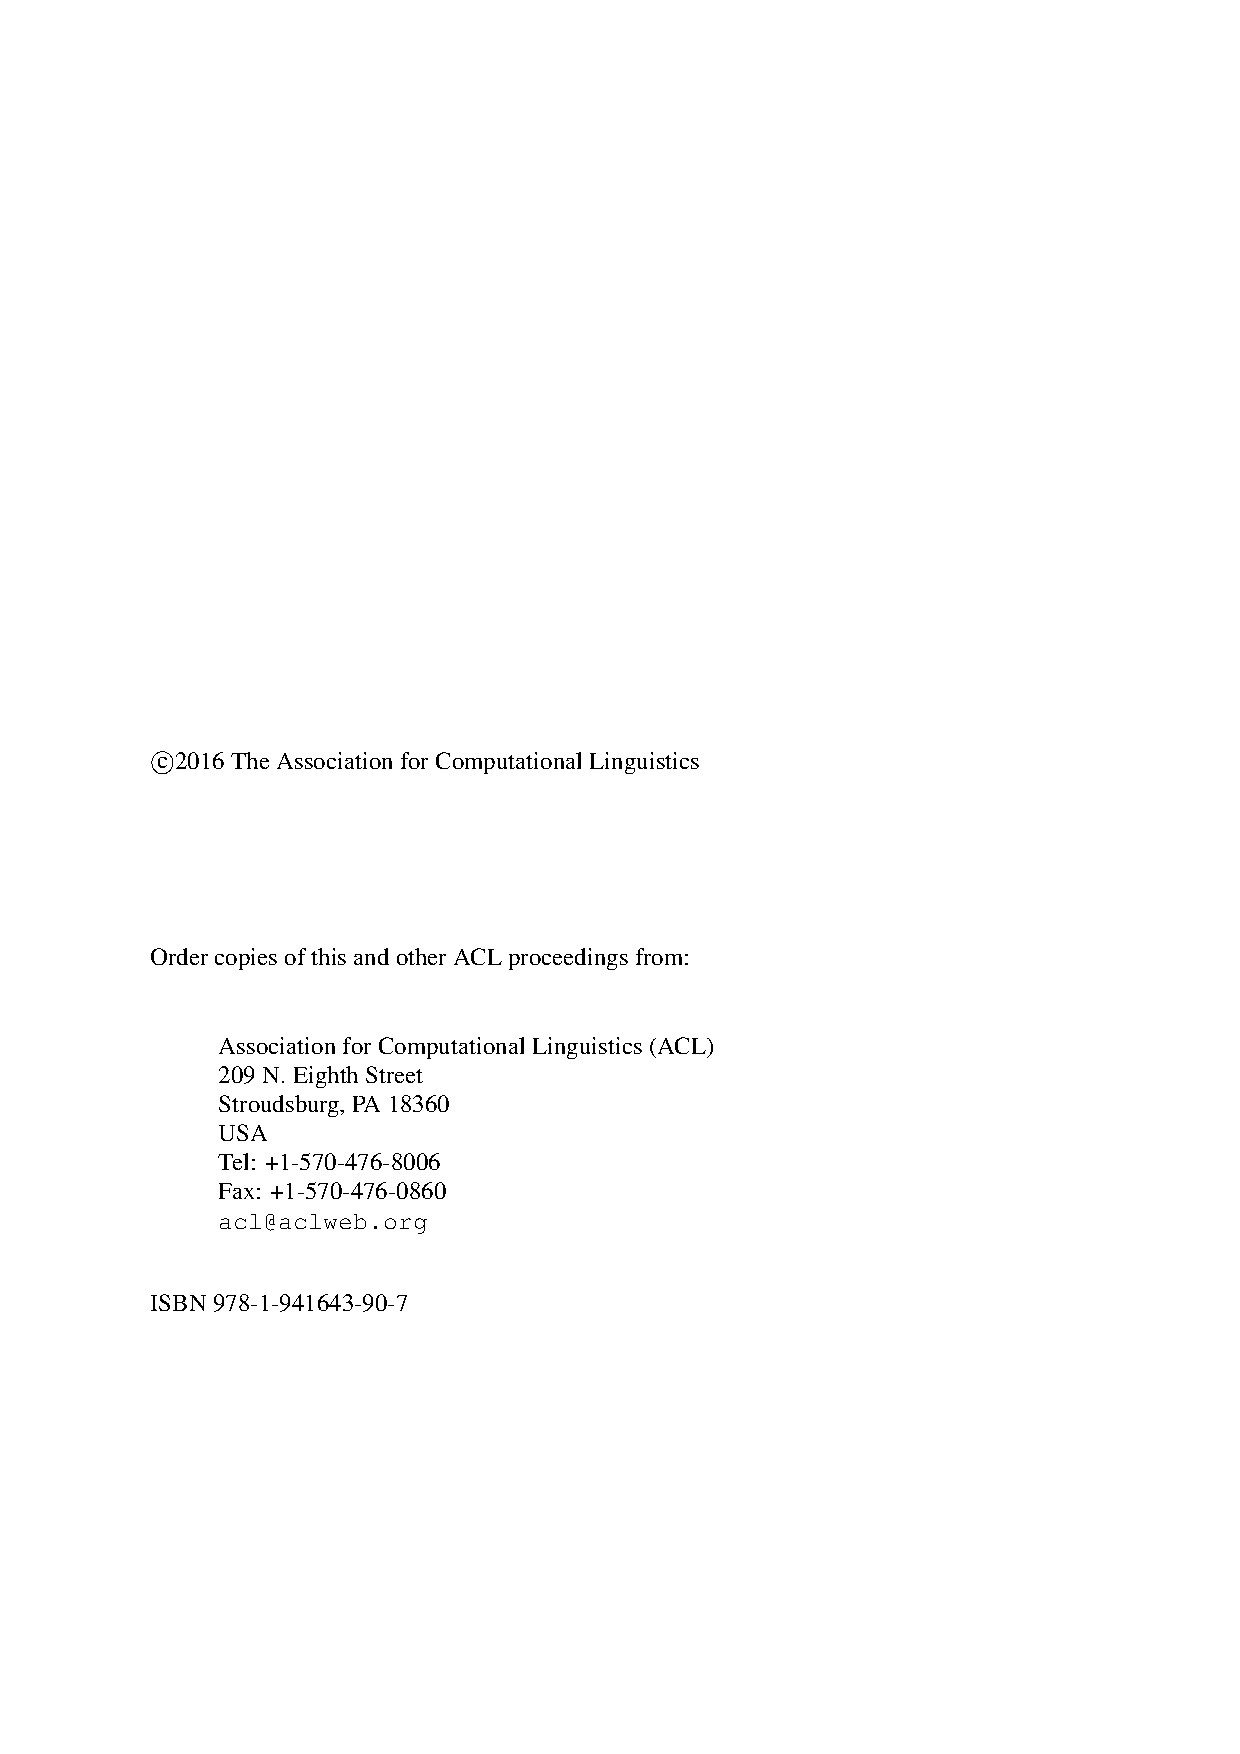
\includepdf{copyright.pdf}

\ifthenelse{\equal{\draftflag}{1}}{\draftframe}{}
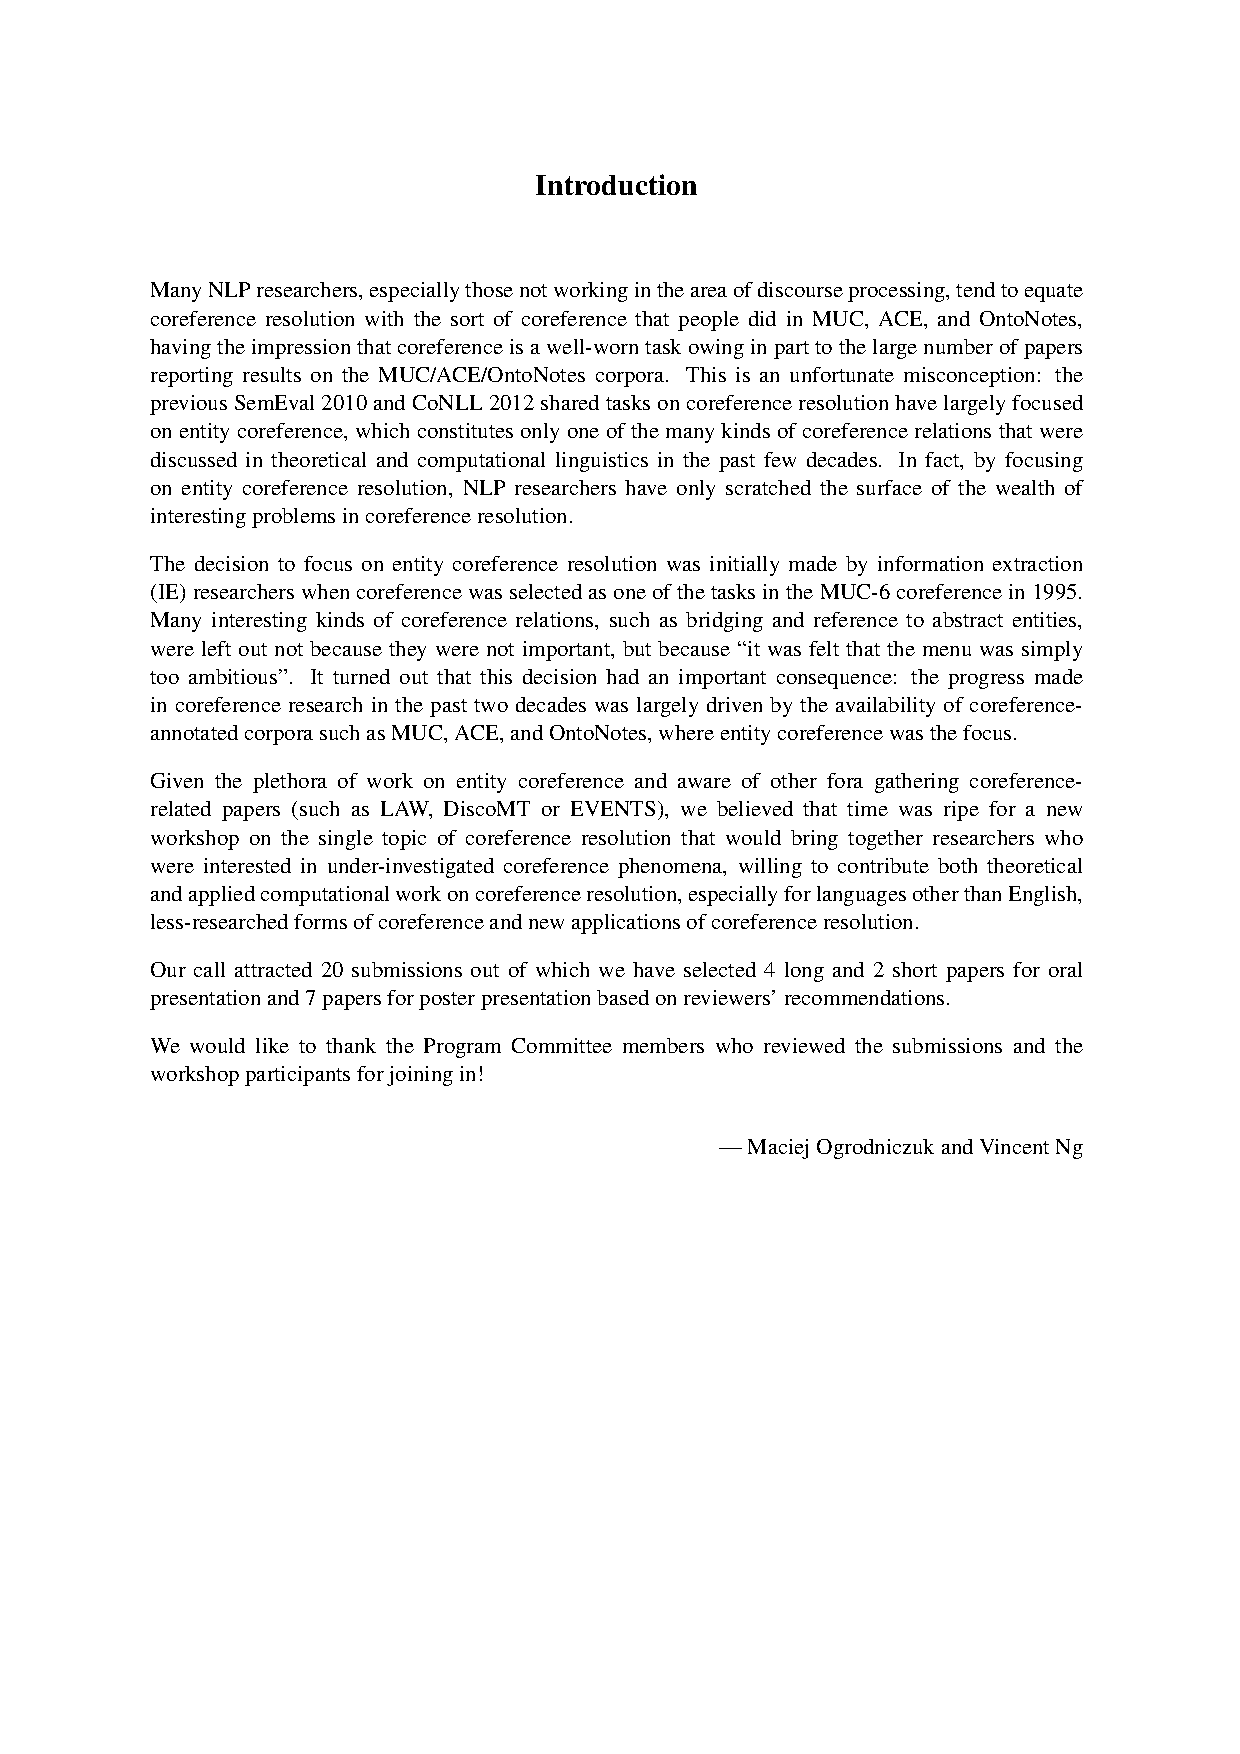
\includepdf{preface.pdf}
\ifthenelse{\isodd{\value{page}}}{}{\newpage \thispagestyle{empty} \phantom{.}}

\ifthenelse{\equal{\draftflag}{1}}{\draftframe}{}

\includepdf{organizers.pdf}
\ifthenelse{\isodd{\value{page}}}{}{\newpage \thispagestyle{empty} \phantom{.}}

\ifthenelse{\equal{\draftflag}{1}}{\draftframe}{}
\setlength{\parindent}{0in}
\setlength{\parskip}{2ex}

\begin{center}
  {\Large \bf Table of Contents}
\end{center}

\vspace*{0.5cm}
\hyperlink{page.1}{\em Sense Anaphoric Pronouns: Am I One?}\samepage \\
\hspace*{7mm} Marta Recasens, Zhichao Hu and Olivia Rhinehart\dotfill \hyperpage{1}

\hyperlink{page.7}{\em Experiments on bridging across languages and genres}\samepage \\
\hspace*{7mm} Yulia Grishina\dotfill \hyperpage{7}

\hyperlink{page.16}{\em Bridging Relations in Polish: Adaptation of Existing Typologies}\samepage \\
\hspace*{7mm} Maciej Ogrodniczuk and Magdalena Zawis{\l}awska\dotfill \hyperpage{16}

\hyperlink{page.23}{\em Beyond Identity Coreference: Contrasting Indicators of Textual Coherence in English and German}\samepage \\
\hspace*{7mm} Kerstin Kunz, Ekaterina Lapshinova-Koltunski and Jos\'{e} Manuel Mart\'{i}nez\dotfill \hyperpage{23}

\hyperlink{page.32}{\em Exploring the steps of Verb Phrase Ellipsis}\samepage \\
\hspace*{7mm} Zhengzhong Liu, Edgar Gonz\`{a}lez Pellicer and Daniel Gillick\dotfill \hyperpage{32}

\hyperlink{page.41}{\em Anaphoricity in Connectives: A Case Study on German}\samepage \\
\hspace*{7mm} Manfred Stede and Yulia Grishina\dotfill \hyperpage{41}

\hyperlink{page.47}{\em Abstract Coreference in a Multilingual Perspective: a View on Czech and German}\samepage \\
\hspace*{7mm} Anna Nedoluzhko and Ekaterina Lapshinova-Koltunski\dotfill \hyperpage{47}

\hyperlink{page.53}{\em Antecedent Prediction Without a Pipeline}\samepage \\
\hspace*{7mm} Sam Wiseman, Alexander M. Rush and Stuart Shieber\dotfill \hyperpage{53}

\hyperlink{page.59}{\em Bridging Corpus for Russian in comparison with Czech}\samepage \\
\hspace*{7mm} Anna Roitberg and Anna Nedoluzhko\dotfill \hyperpage{59}

\hyperlink{page.67}{\em Coreference Resolution for the Basque Language with BART}\samepage \\
\hspace*{7mm} Ander Soraluze, Olatz Arregi, Xabier Arregi, Arantza Diaz de Ilarraza, Mijail Kabadjov\\
\hspace*{7mm} and Massimo Poesio\dotfill \hyperpage{67}

\hyperlink{page.74}{\em Error analysis for anaphora resolution in Russian: new challenging issues for anaphora resolution task in a morphologically rich language}\samepage \\
\hspace*{7mm} Svetlana Toldova, Ilya Azerkovich, Alina Ladygina, Anna Roitberg and Maria Vasilyeva\dotfill \hyperpage{74}

\hyperlink{page.84}{\em How to Handle Split Antecedents in Tamil?}\samepage \\
\hspace*{7mm} Vijay Sundar Ram and Sobha Lalitha Devi\dotfill \hyperpage{84}

\hyperlink{page.92}{\em When Annotation Schemes Change Rules Help:  A Configurable Approach to Coreference Resolution beyond OntoNotes}\samepage \\
\hspace*{7mm} Amir Zeldes and Shuo Zhang\dotfill \hyperpage{92}

\ifthenelse{\isodd{\value{page}}}{}{\newpage \thispagestyle{empty} \phantom{.}}

\ifthenelse{\equal{\draftflag}{1}}{\draftframe}{}
\addcontentsline{toc}{chapter}{Program}
\setlength{\parindent}{0in}
\setlength{\parskip}{2ex}
\renewcommand{\baselinestretch}{0.87}

\begin{center}
{\Large \bf
  Workshop Program: June 16, 2016
}
\end{center}
\vspace{3mm}
\begin{tabular}{p{20mm}p{128mm}}
{\bf Session 1} \\
\\
09:00--09:10 & {\em Introduction} \\
\\
09:10--10:10 & {\em Invited talk} \\[5pt]
         & \em{The (Non)Utility of Semantics for Coreference Resolution (CORBON Remix)} \\
         & Michael Strube\\
\\
10:10--10:30 & \hyperlink{page.1}{\em Sense Anaphoric Pronouns: Am I One?}\\
         & Marta Recasens, Zhichao Hu and Olivia Rhinehart \\
\\
\\ & {\bf\em Coffee break} \\[1pt]
\\[1pt]
\\
{\bf Session 2} \\
\\
11:00--11:30 & \hyperlink{page.7}{\em Experiments on Bridging Across Languages and Genres}\\
         & Yulia Grishina \\
\\

11:30--12:00 & \hyperlink{page.16}{\em Bridging Relations in Polish: Adaptation of Existing Typologies}\\
         & Maciej Ogrodniczuk and Magdalena Zawis{\l}awska \\
\\

12:00--12:30 & \hyperlink{page.23}{\em Beyond Identity Coreference: Contrasting Indicators of Textual Coherence} \\
             & \em{in English and German}\\
         & Kerstin Kunz, Ekaterina Lapshinova-Koltunski and Jos\'{e} Manuel Mart\'{i}nez \\
\\

\\ & {\bf\em Lunch break} \\[1pt]
\\[1pt]
\\
{\bf Session 3} \\
\\
14:00--15:00 & {\em Invited talk}\\[5
pt]
         & \em{A Bayesian Model of Pronoun Production and Interpretation}\\
         & Andrew Kehler\\
\\
15:00--15:30 & \hyperlink{page.32}{\em Exploring the Steps of Verb Phrase Ellipsis}\\
         & Zhengzhong Liu, Edgar Gonz\`{a}lez Pellicer and Daniel Gillick \\
\\[5pt]

\\ & {\bf\em Coffee break} \\
\end{tabular}
\newpage
\begin{tabular}{p{20mm}p{128mm}}
{\bf Session 4} \\
\\
16:00--16:20 & \hyperlink{page.41}{\em Anaphoricity in Connectives: A Case Study on German}\\
         & Manfred Stede and Yulia Grishina \\
\\

16:20--16:30 & {\em One minute madness for posters} \\
\\
16:30--17:30 & {\em Poster session} \\
\\
 & \hyperlink{page.47}{\em Abstract Coreference in a Multilingual Perspective: a View on Czech and German}\\
         & Anna Nedoluzhko and Ekaterina Lapshinova-Koltunski \\
\\

 & \hyperlink{page.53}{\em Antecedent Prediction Without a Pipeline}\\
         & Sam Wiseman, Alexander M. Rush and Stuart Shieber \\
\\

 & \hyperlink{page.59}{\em Bridging Corpus for Russian in Comparison with Czech}\\
         & Anna Roitberg and Anna Nedoluzhko \\
\\

 & \hyperlink{page.67}{\em Coreference Resolution for the Basque Language with BART}\\
         & Ander Soraluze, Olatz Arregi, Xabier Arregi, Arantza Diaz de Ilarraza, Mijail Kabadjov and Massimo Poesio \\
\\

 & \hyperlink{page.74}{\em Error Analysis for Anaphora Resolution in Russian: New Challenging Issues for Anaphora Resolution Task in a Morphologically Rich Language}\\
         & Svetlana Toldova, Ilya Azerkovich, Alina Ladygina, Anna Roitberg and Maria Vasilyeva \\
\\

 & \hyperlink{page.84}{\em How to Handle Split Antecedents in Tamil?}\\
         & Vijay Sundar Ram and Sobha Lalitha Devi \\
\\

 & \hyperlink{page.92}{\em When Annotation Schemes Change Rules Help: A Configurable Approach to Coreference Resolution beyond OntoNotes}\\
         & Amir Zeldes and Shuo Zhang \\
\\


\end{tabular}

\ifthenelse{\isodd{\value{page}}}{}{\newpage \thispagestyle{empty} \phantom{.}}

% -------- INCLUDED PAPERS --------

\newpage
\pagenumbering{arabic}
\setcounter{page}{1}
\ClearShipoutPicture
\index{Recasens, Marta}
\index{Hu, Zhichao}
\index{Rhinehart, Olivia}
\citeinfo{1}{6}
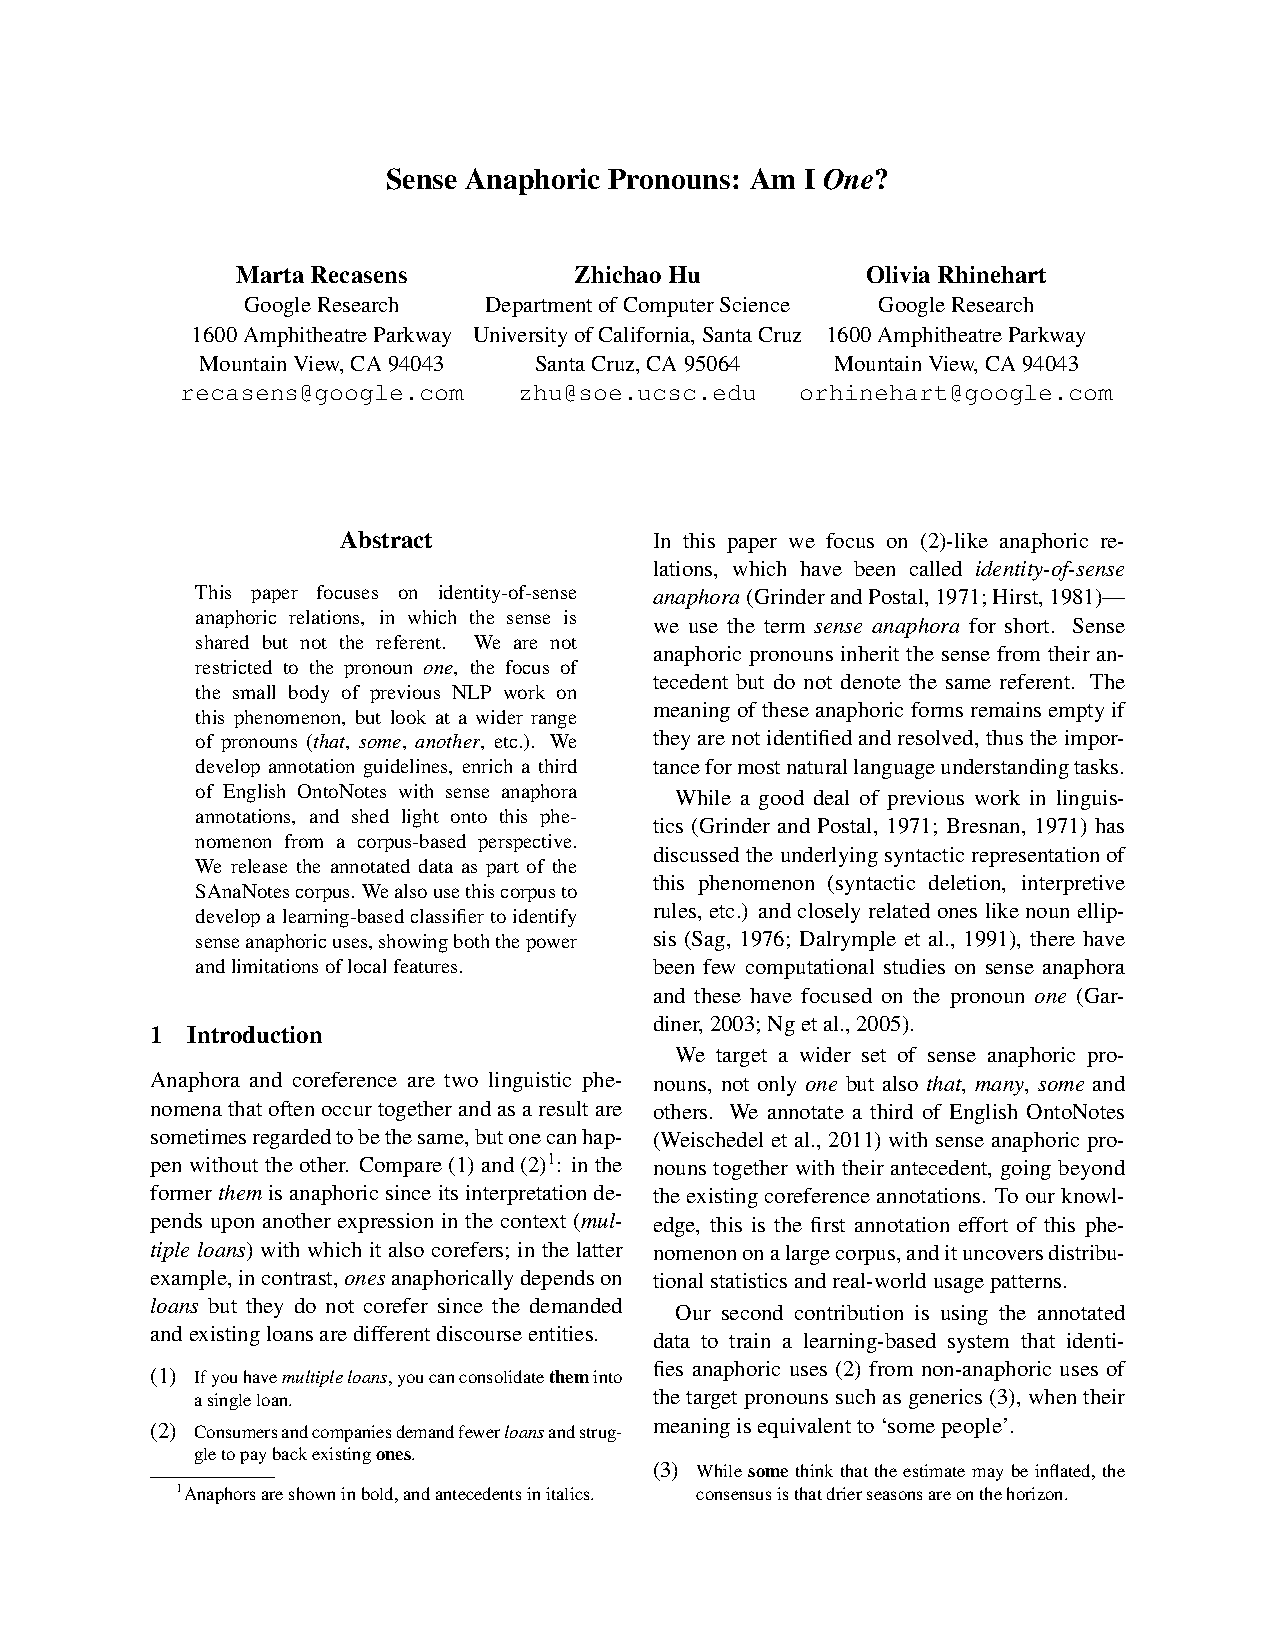
\includepdf[pages=1,offset=0mm 5mm,addtotoc={1,chapter,1,{Sense Anaphoric Pronouns: Am I One?},ref:paper_14}]{final/14/14_Paper.pdf}
\ClearShipoutPicture
\includepdf[pages=2-,offset=0mm 5mm]{final/14/14_Paper.pdf}
\index{Grishina, Yulia}
\citeinfo{7}{15}
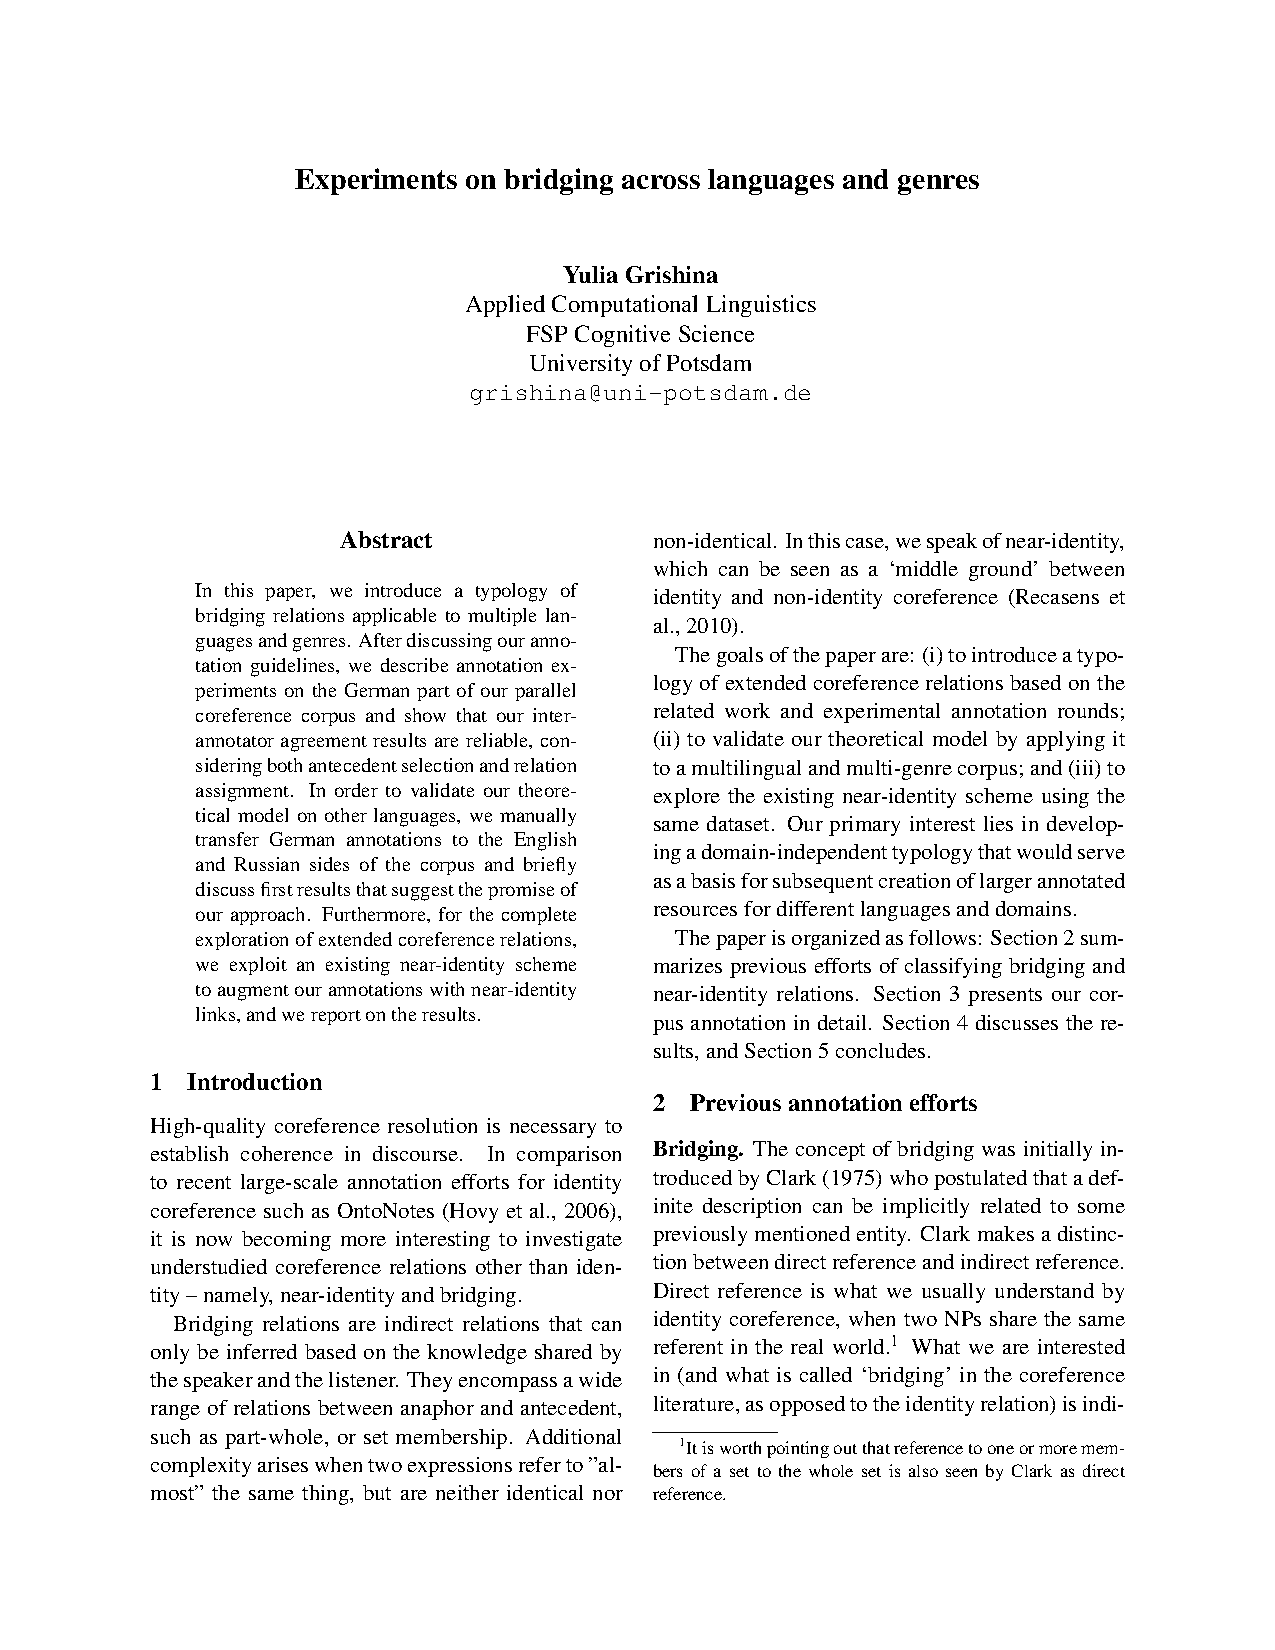
\includepdf[pages=1,offset=0mm 5mm,addtotoc={1,chapter,1,{Experiments on bridging across languages and genres},ref:paper_17}]{final/17/17_Paper.pdf}
\ClearShipoutPicture
\includepdf[pages=2-,offset=0mm 5mm]{final/17/17_Paper.pdf}
\index{Ogrodniczuk, Maciej}
\index{Zawisawska, Magdalena@Zawis{\l}awska, Magdalena}
\citeinfo{16}{22}
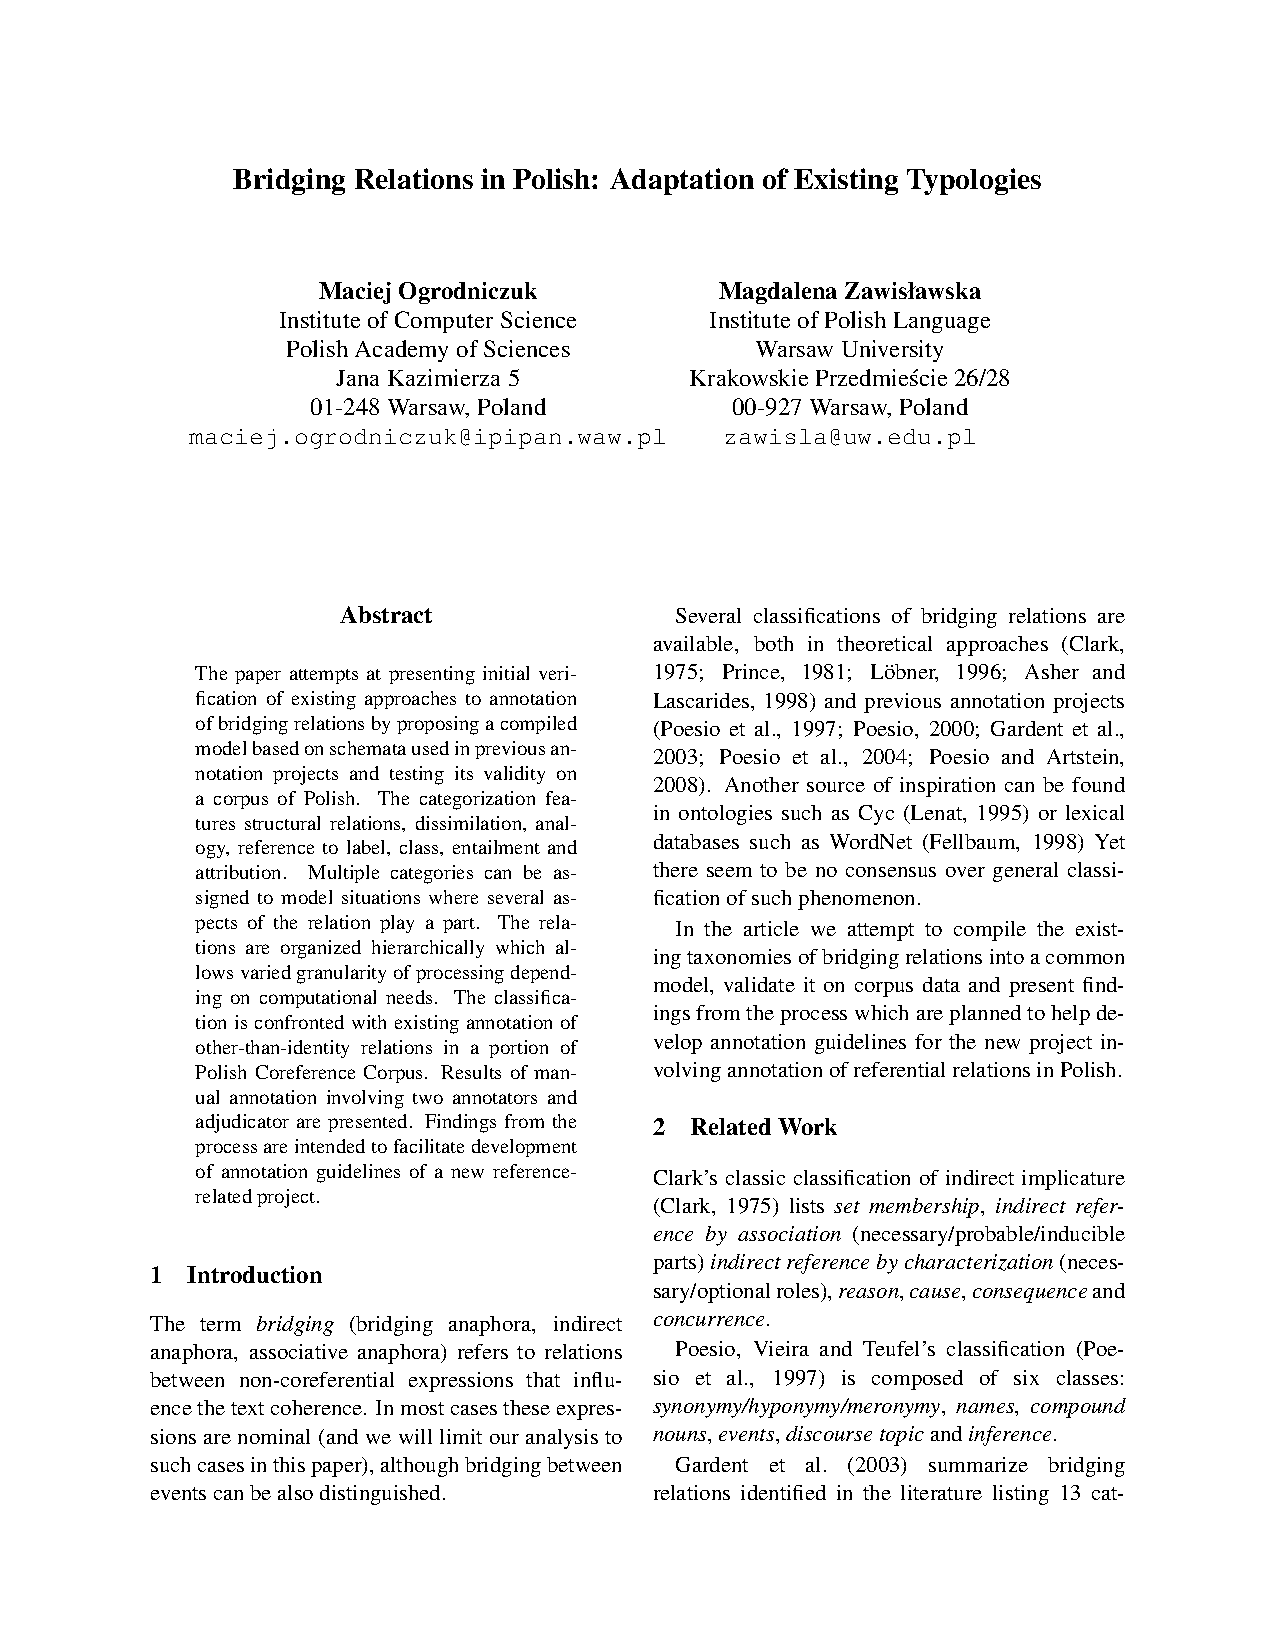
\includepdf[pages=1,addtotoc={1,chapter,1,{Bridging Relations in Polish: Adaptation of Existing Typologies},ref:paper_21}]{final/21/21_Paper.pdf}
\ClearShipoutPicture
\includepdf[pages=2-]{final/21/21_Paper.pdf}
\index{Kunz, Kerstin}
\index{Lapshinova-Koltunski, Ekaterina}
\index{Martinez, Jose Manuel@Mart\'{i}nez, Jos\'{e} Manuel}
\citeinfo{23}{31}
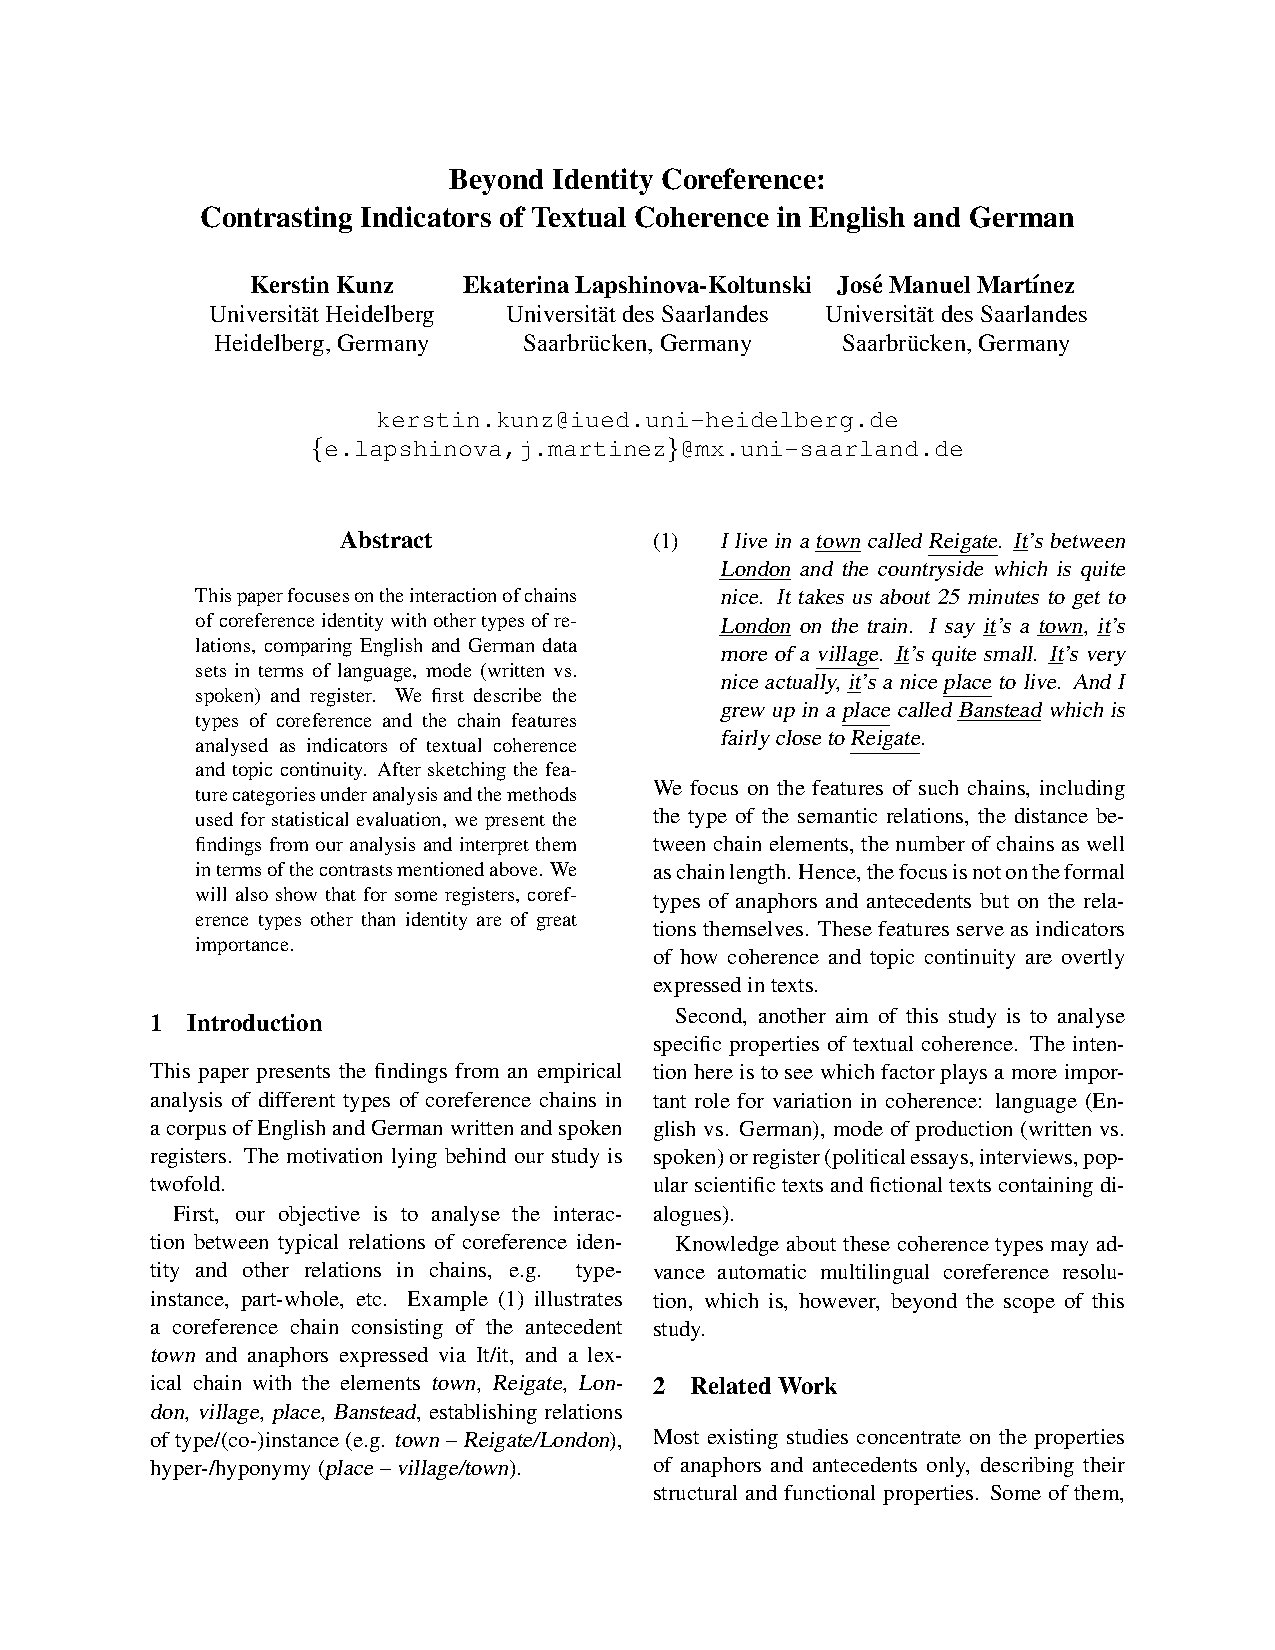
\includepdf[pages=1,addtotoc={1,chapter,1,{Beyond Identity Coreference: Contrasting Indicators of Textual Coherence in English and German},ref:paper_6}]{final/6/6_Paper.pdf}
\ClearShipoutPicture
\includepdf[pages=2-]{final/6/6_Paper.pdf}
\index{Liu, Zhengzhong}
\index{Gonzalez Pellicer, Edgar@Gonz\`{a}lez Pellicer, Edgar}
\index{Gillick, Daniel}
\citeinfo{32}{40}
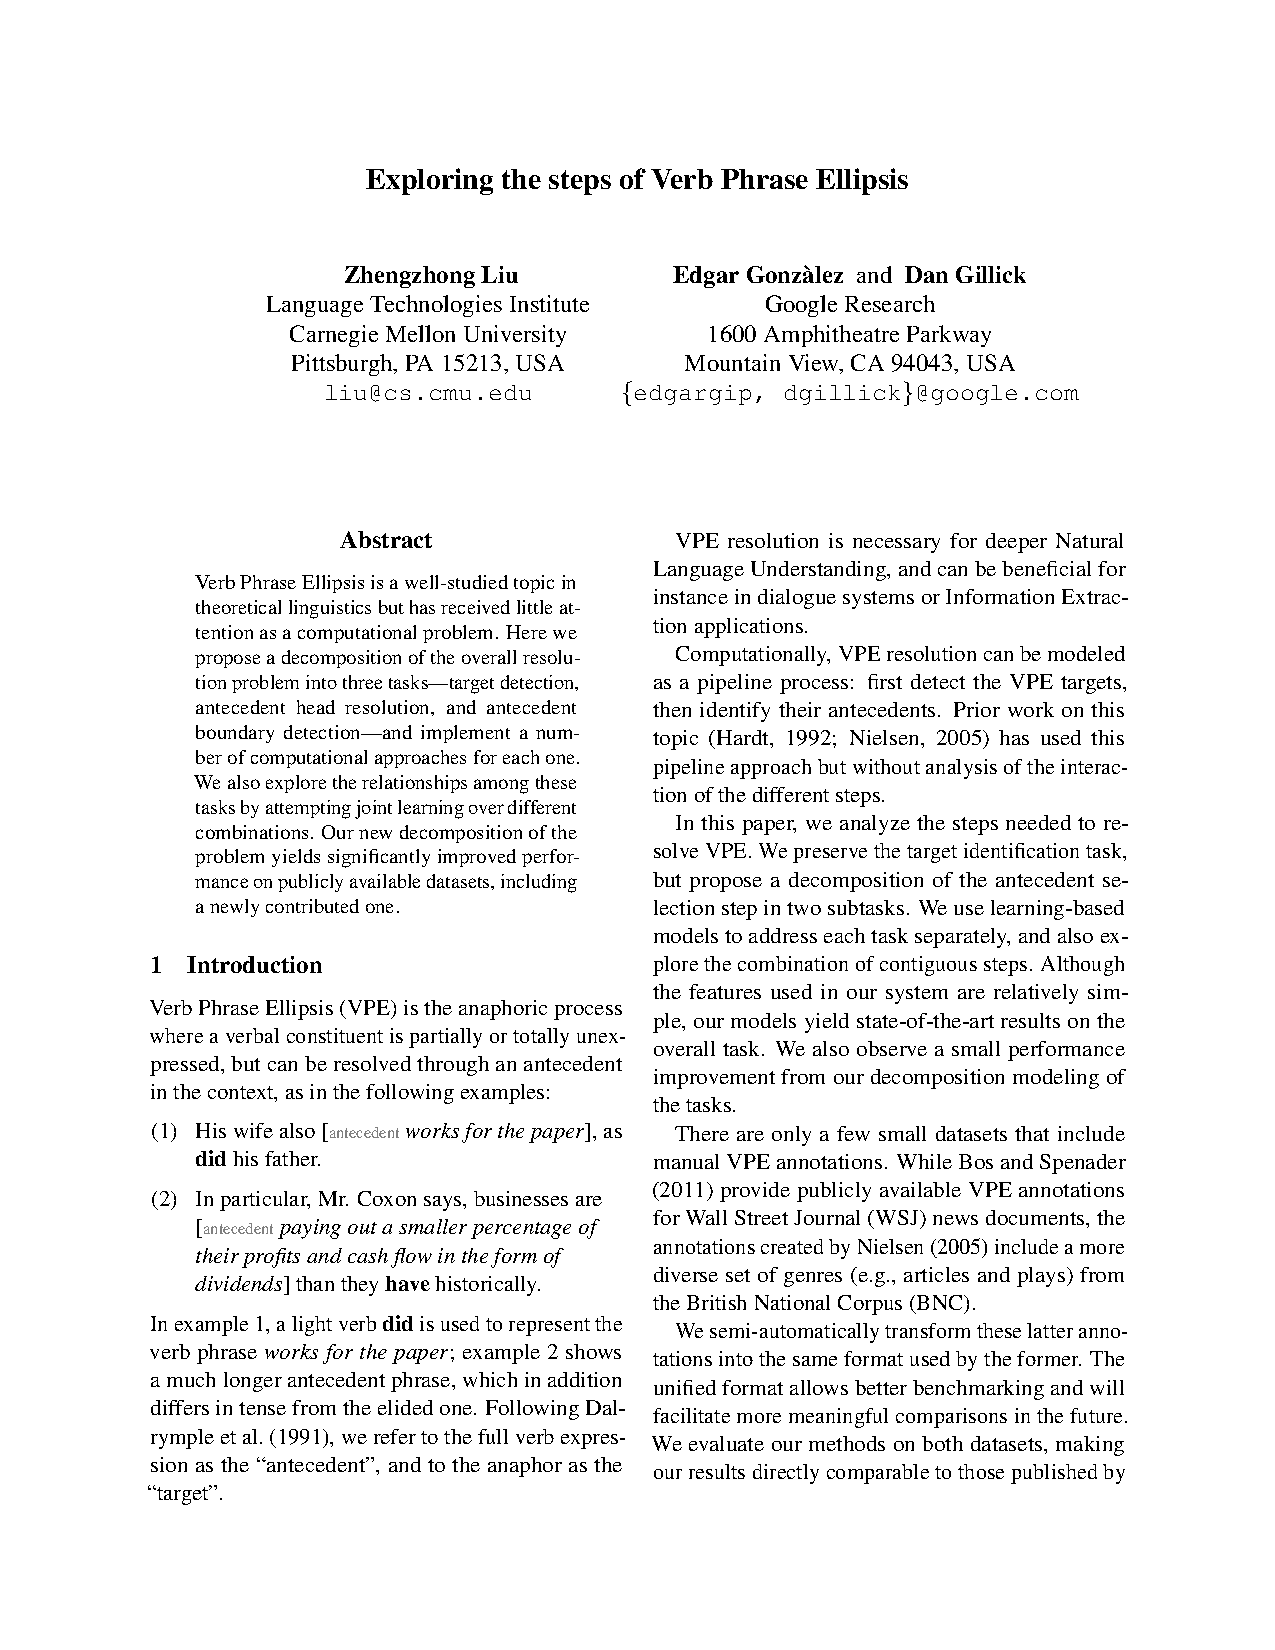
\includepdf[pages=1,addtotoc={1,chapter,1,{Exploring the steps of Verb Phrase Ellipsis},ref:paper_19}]{final/19/19_Paper.pdf}
\ClearShipoutPicture
\includepdf[pages=2-]{final/19/19_Paper.pdf}
\index{Stede, Manfred}
\index{Grishina, Yulia}
\citeinfo{41}{46}
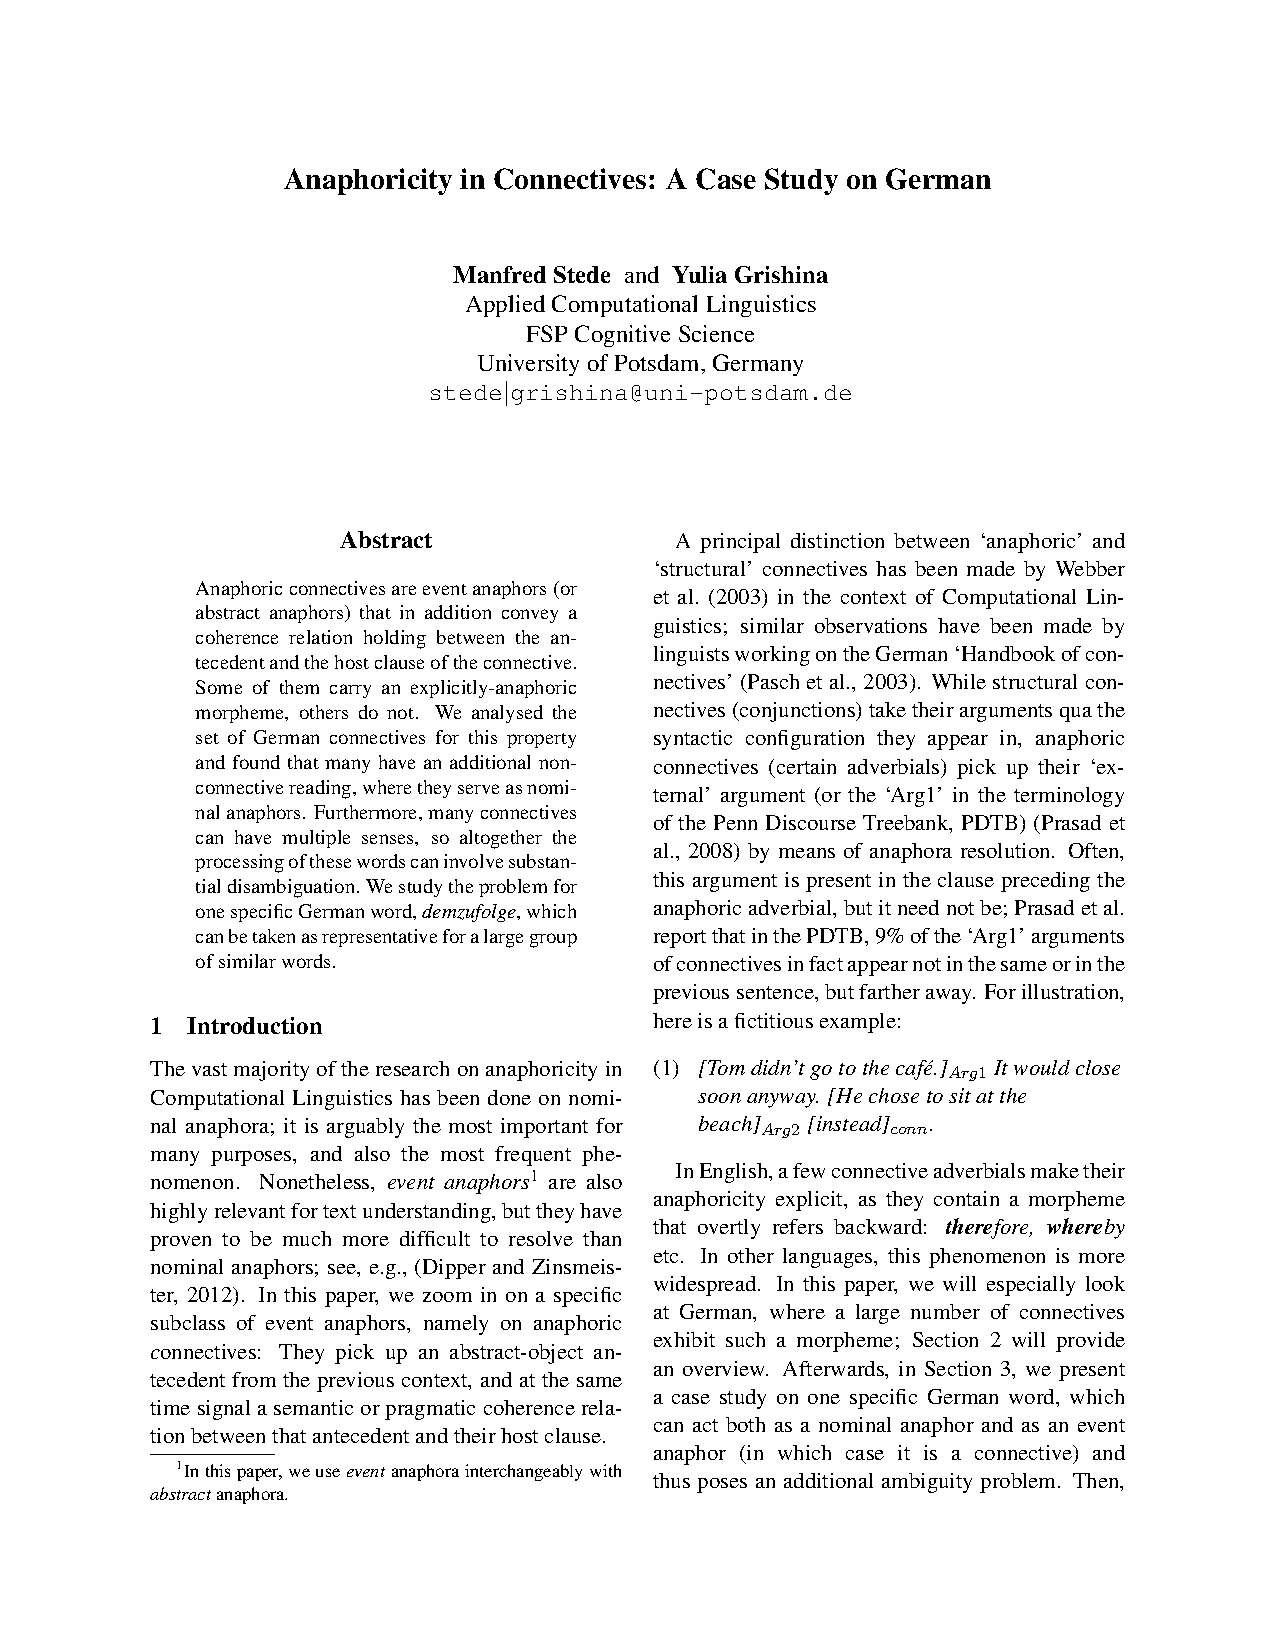
\includepdf[pages=1,addtotoc={1,chapter,1,{Anaphoricity in Connectives: A Case Study on German},ref:paper_16}]{final/16/16_Paper.pdf}
\ClearShipoutPicture
\includepdf[pages=2-]{final/16/16_Paper.pdf}
\index{Nedoluzhko, Anna}
\index{Lapshinova-Koltunski, Ekaterina}
\citeinfo{47}{52}
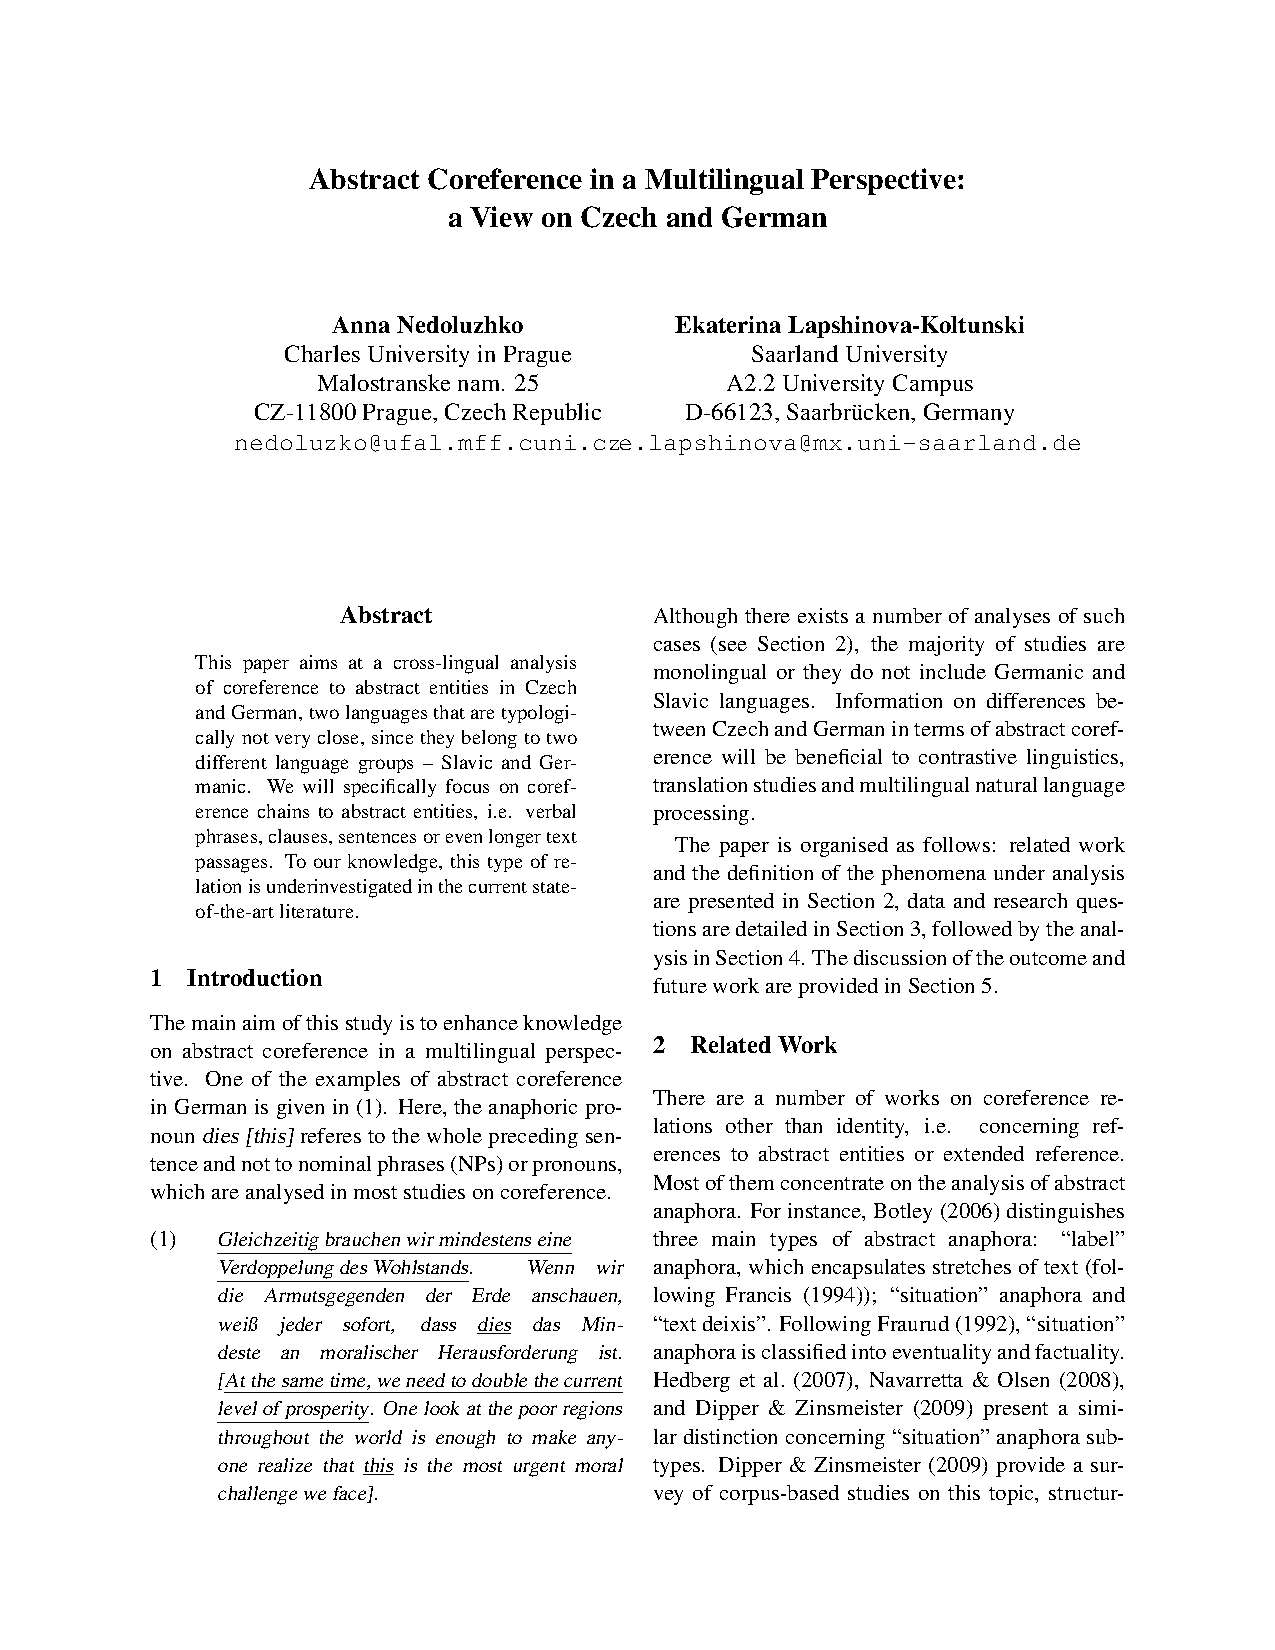
\includepdf[pages=1,addtotoc={1,chapter,1,{Abstract Coreference in a Multilingual Perspective: a View on Czech and German},ref:paper_3}]{final/3/3_Paper.pdf}
\ClearShipoutPicture
\includepdf[pages=2-]{final/3/3_Paper.pdf}
\index{Wiseman, Sam}
\index{Rush, Alexander M.}
\index{Shieber, Stuart}
\citeinfo{53}{58}
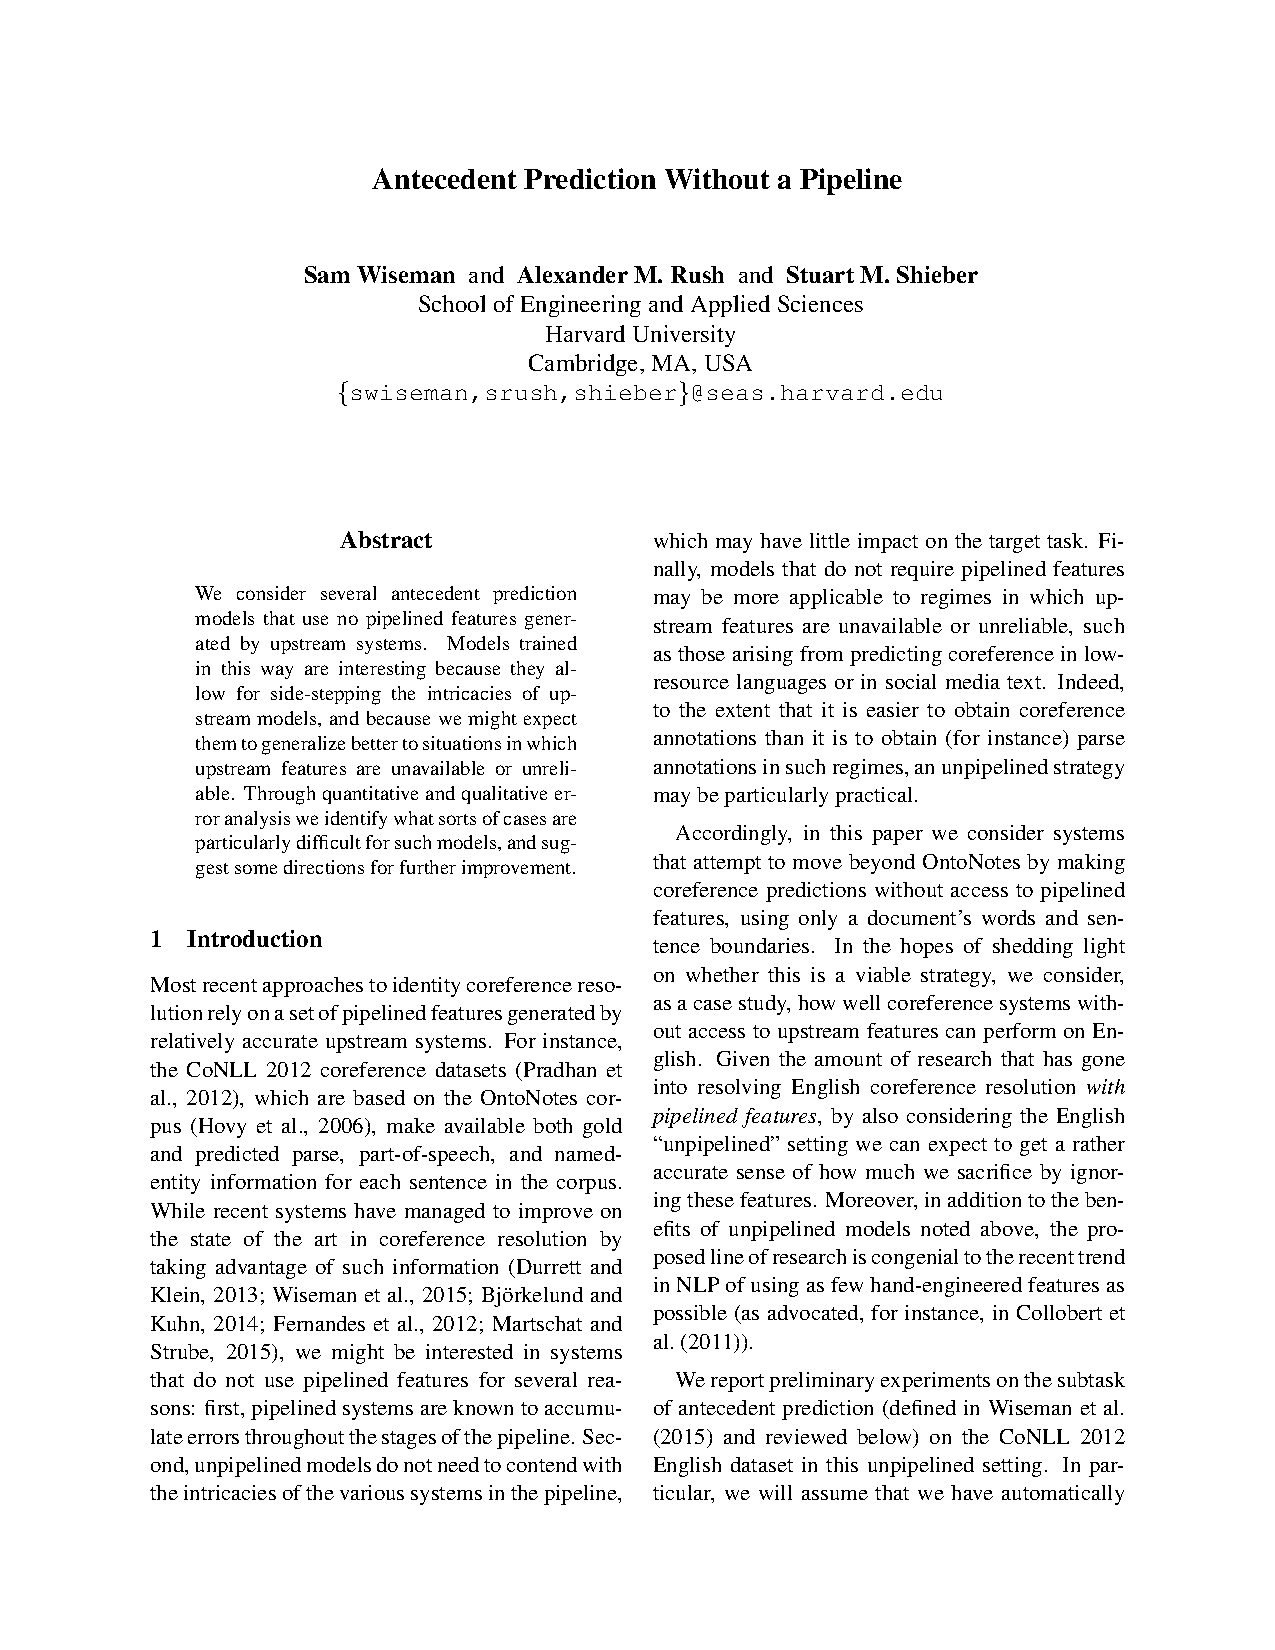
\includepdf[pages=1,offset=0mm 4mm,addtotoc={1,chapter,1,{Antecedent Prediction Without a Pipeline},ref:paper_12}]{final/12/12_Paper.pdf}
\ClearShipoutPicture
\includepdf[pages=2-,offset=0mm 4mm]{final/12/12_Paper.pdf}
\index{Roitberg, Anna}
\index{Nedoluzhko, Anna}
\citeinfo{59}{66}
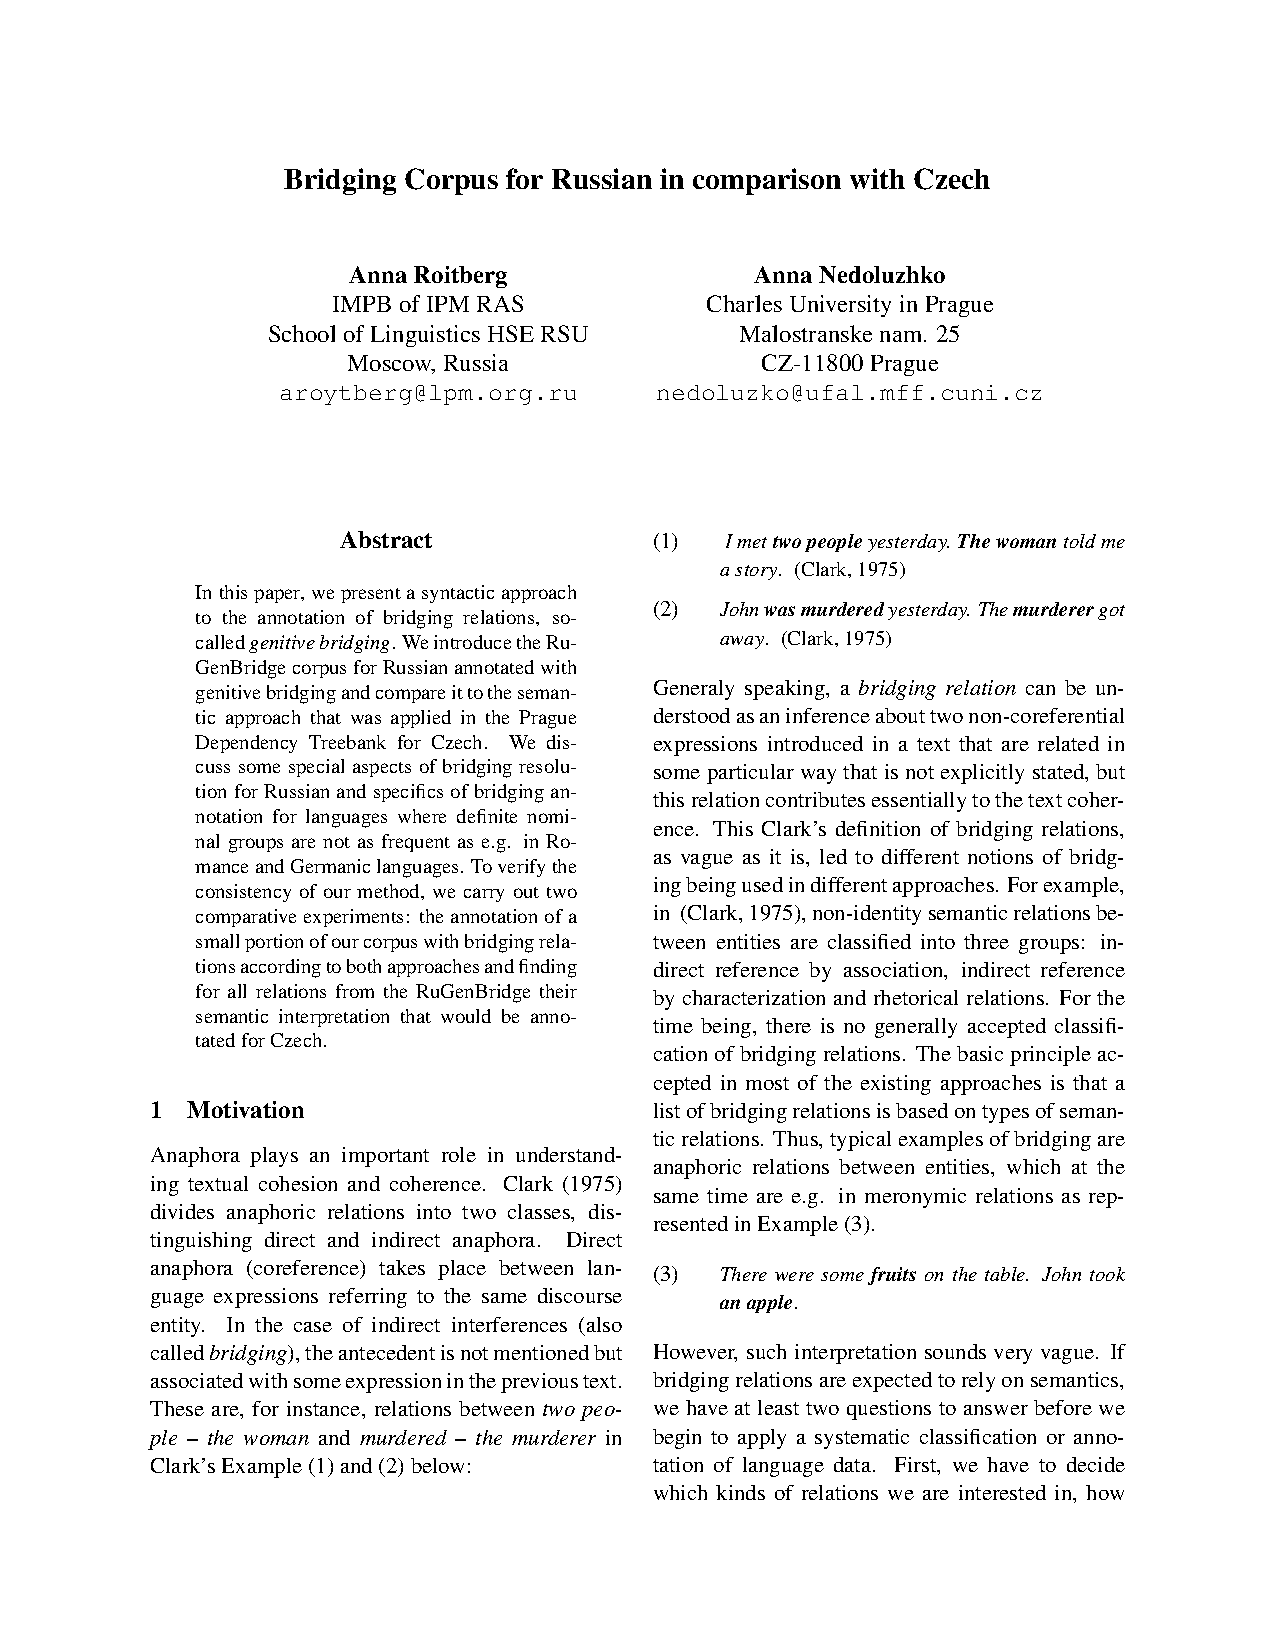
\includepdf[pages=1,addtotoc={1,chapter,1,{Bridging Corpus for Russian in comparison with Czech},ref:paper_5}]{final/5/5_Paper.pdf}
\ClearShipoutPicture
\includepdf[pages=2-]{final/5/5_Paper.pdf}
\index{Soraluze, Ander}
\index{Arregi, Olatz}
\index{Arregi, Xabier}
\index{Diaz de Ilarraza, Arantza}
\index{Kabadjov, Mijail}
\index{Poesio, Massimo}
\citeinfo{67}{73}
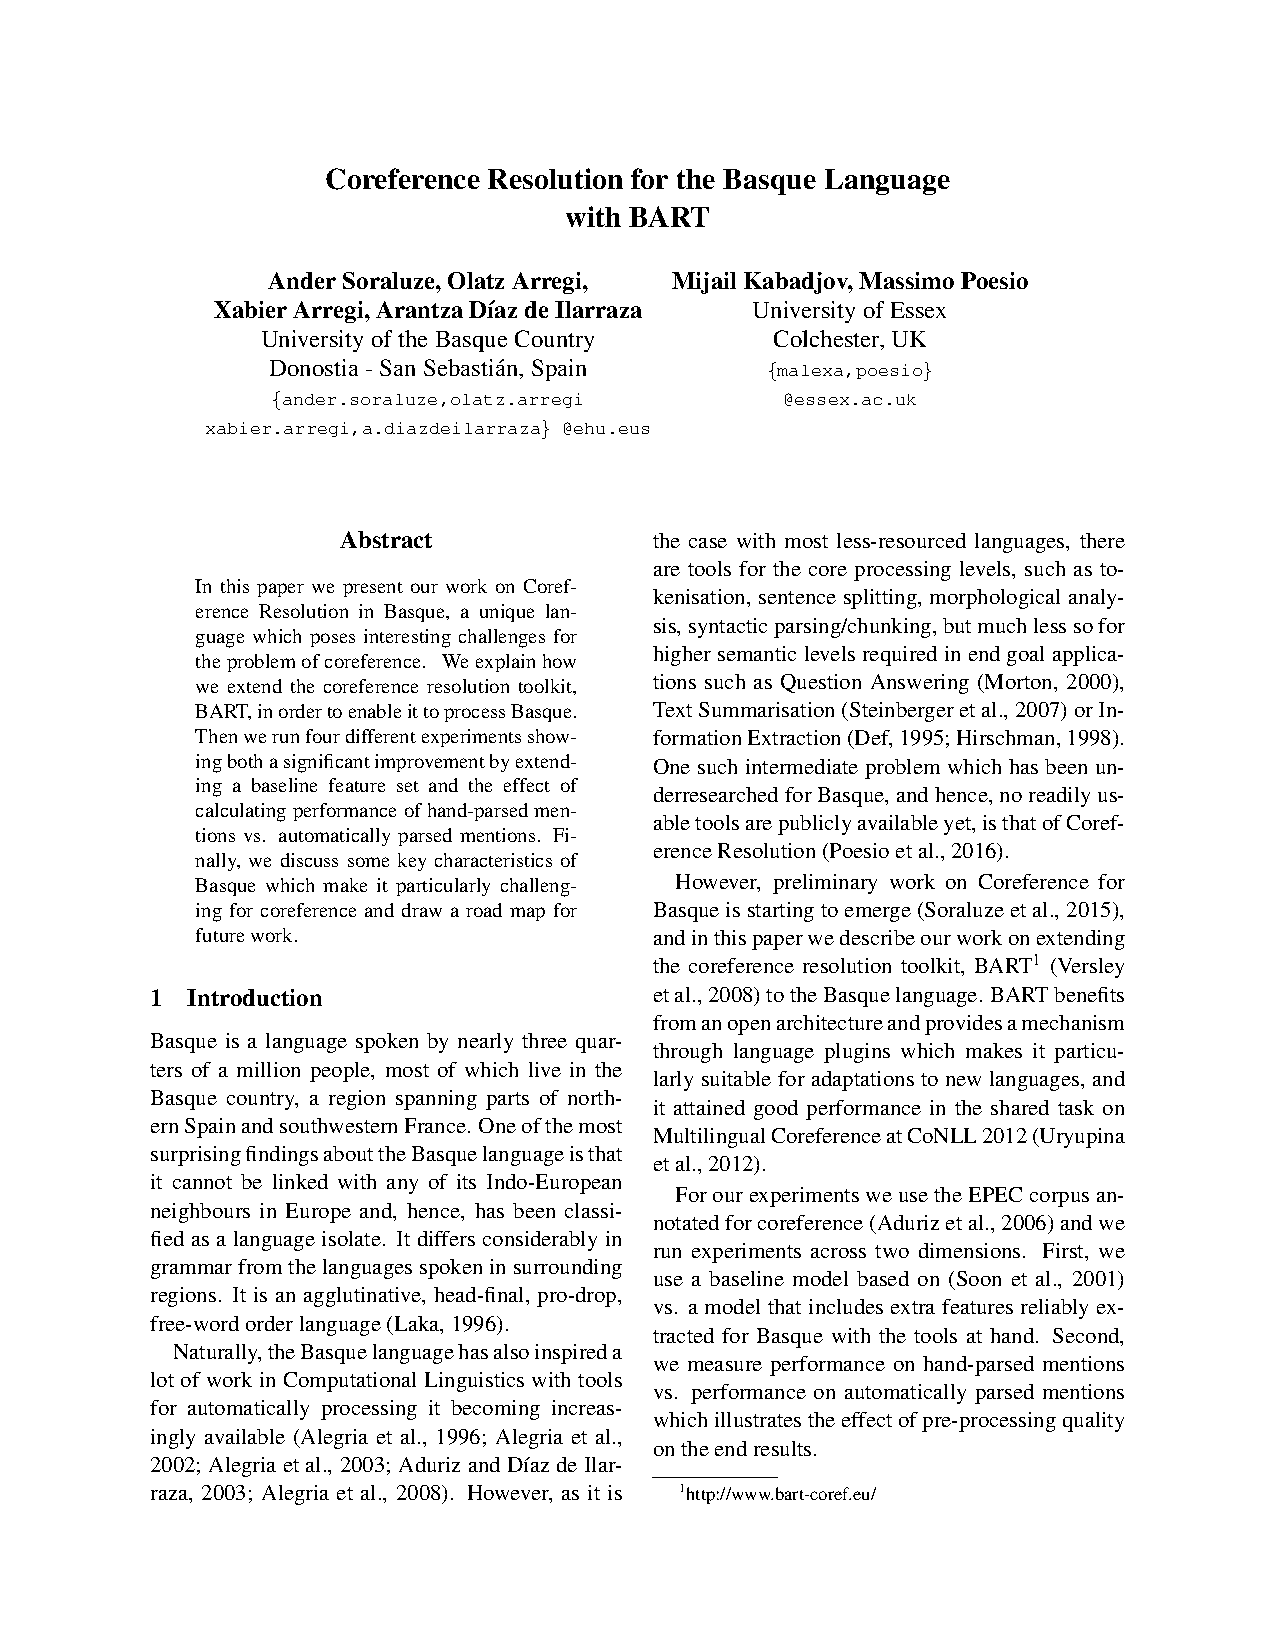
\includepdf[pages=1,addtotoc={1,chapter,1,{Coreference Resolution for the Basque Language with BART},ref:paper_10}]{final/10/10_Paper.pdf}
\ClearShipoutPicture
\includepdf[pages=2-]{final/10/10_Paper.pdf}
\index{Toldova, Svetlana}
\index{Azerkovich, Ilya}
\index{Ladygina, Alina}
\index{Roitberg, Anna}
\index{Vasilyeva, Maria}
\citeinfo{74}{83}
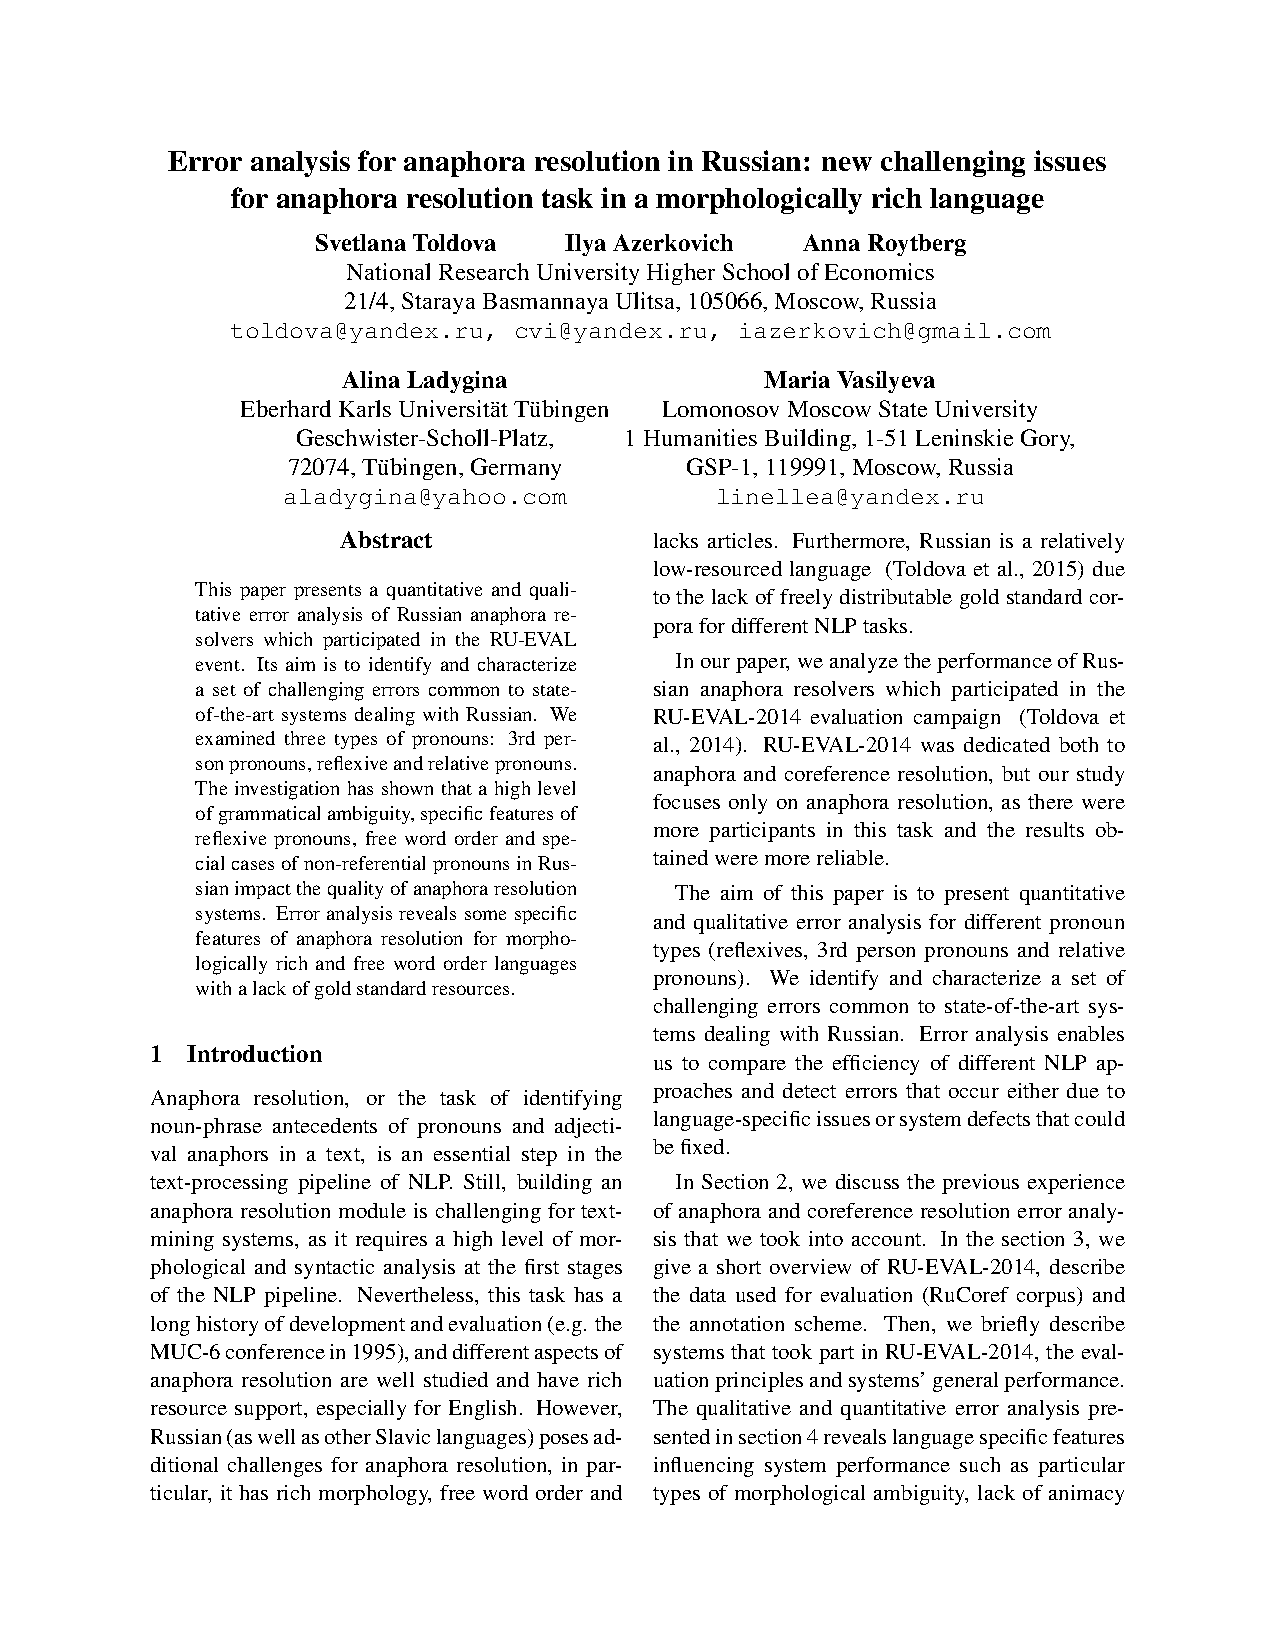
\includepdf[pages=1,addtotoc={1,chapter,1,{Error analysis for anaphora resolution in Russian: new challenging issues for anaphora resolution task in a morphologically rich language},ref:paper_11}]{final/11/11_Paper.pdf}
\ClearShipoutPicture
\includepdf[pages=2-]{final/11/11_Paper.pdf}
\index{Sundar Ram, Vijay}
\index{Lalitha Devi, Sobha}
\citeinfo{84}{91}
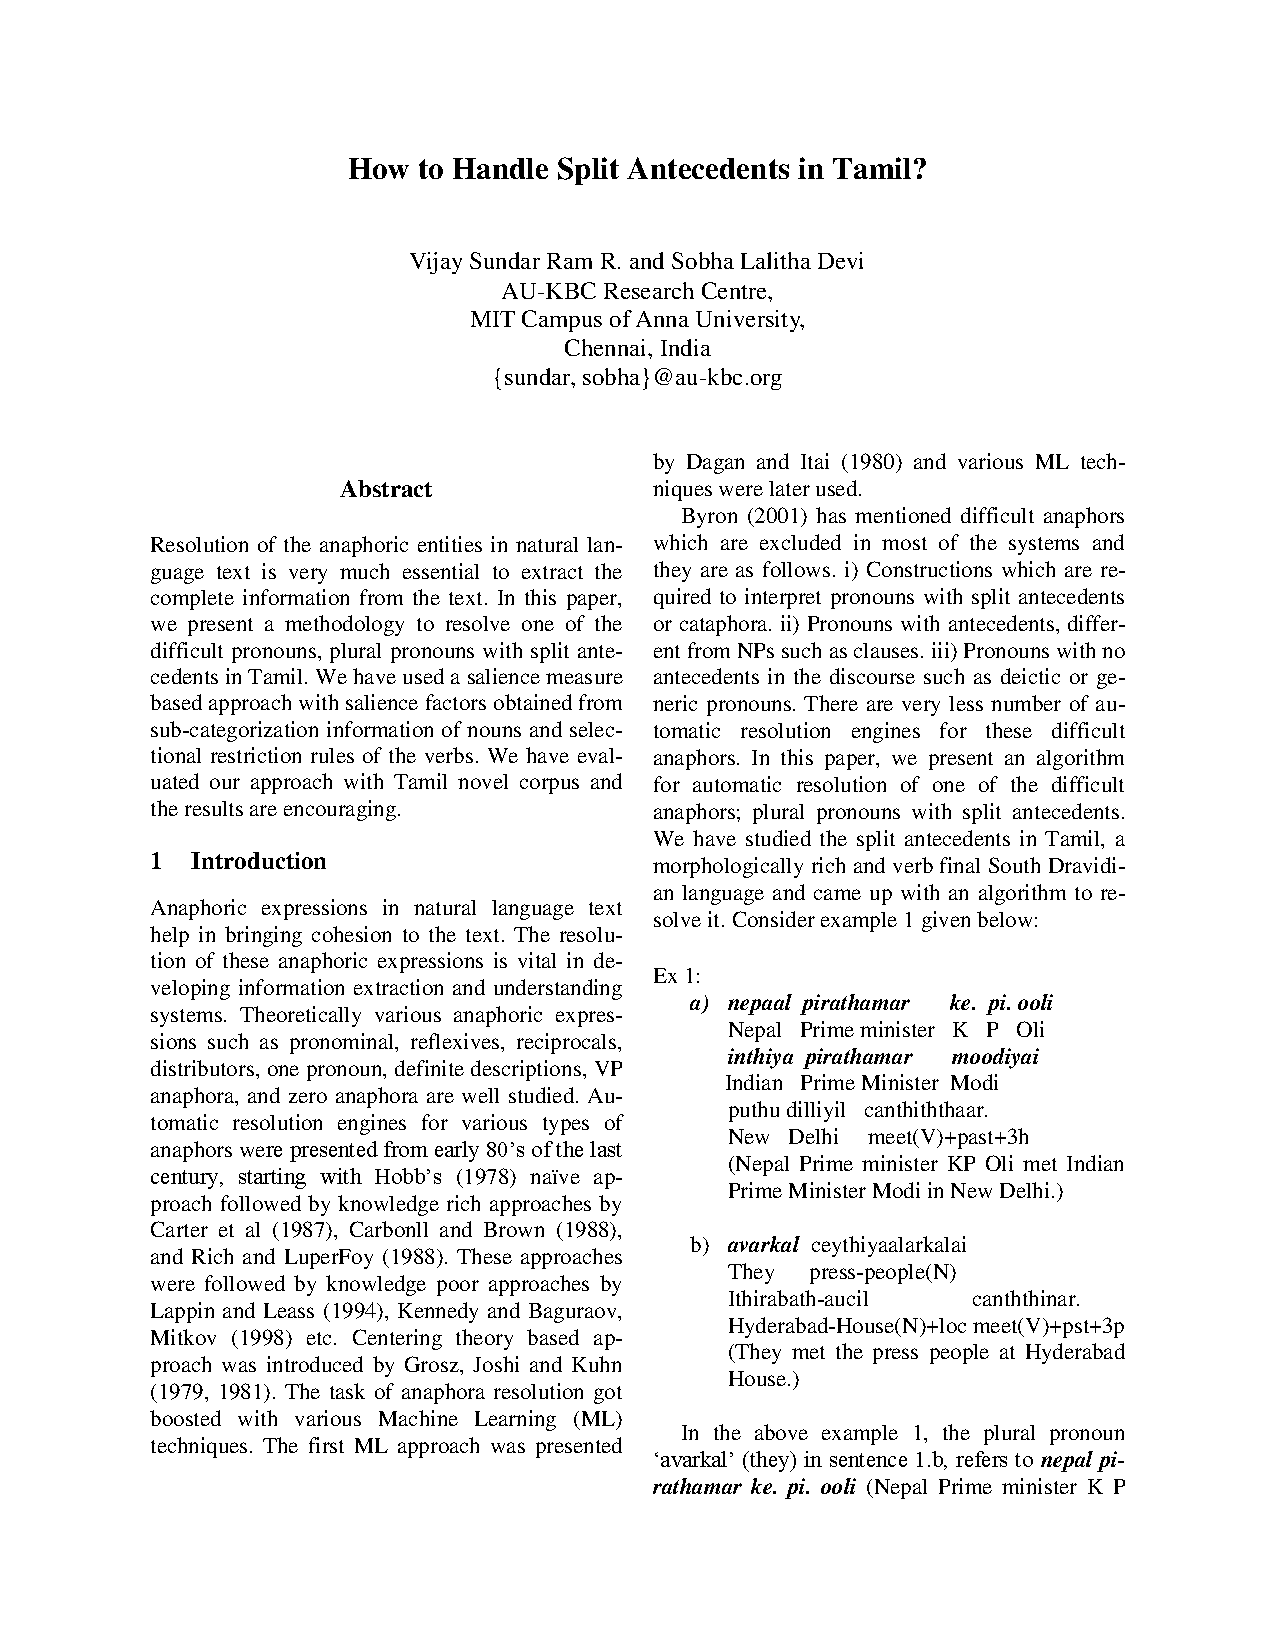
\includepdf[pages=1,addtotoc={1,chapter,1,{How to Handle Split Antecedents in Tamil?},ref:paper_20}]{final/20/20_Paper.pdf}
\ClearShipoutPicture
\includepdf[pages=2-]{final/20/20_Paper.pdf}
\index{Zeldes, Amir}
\index{Zhang, Shuo}
\citeinfo{92}{101}
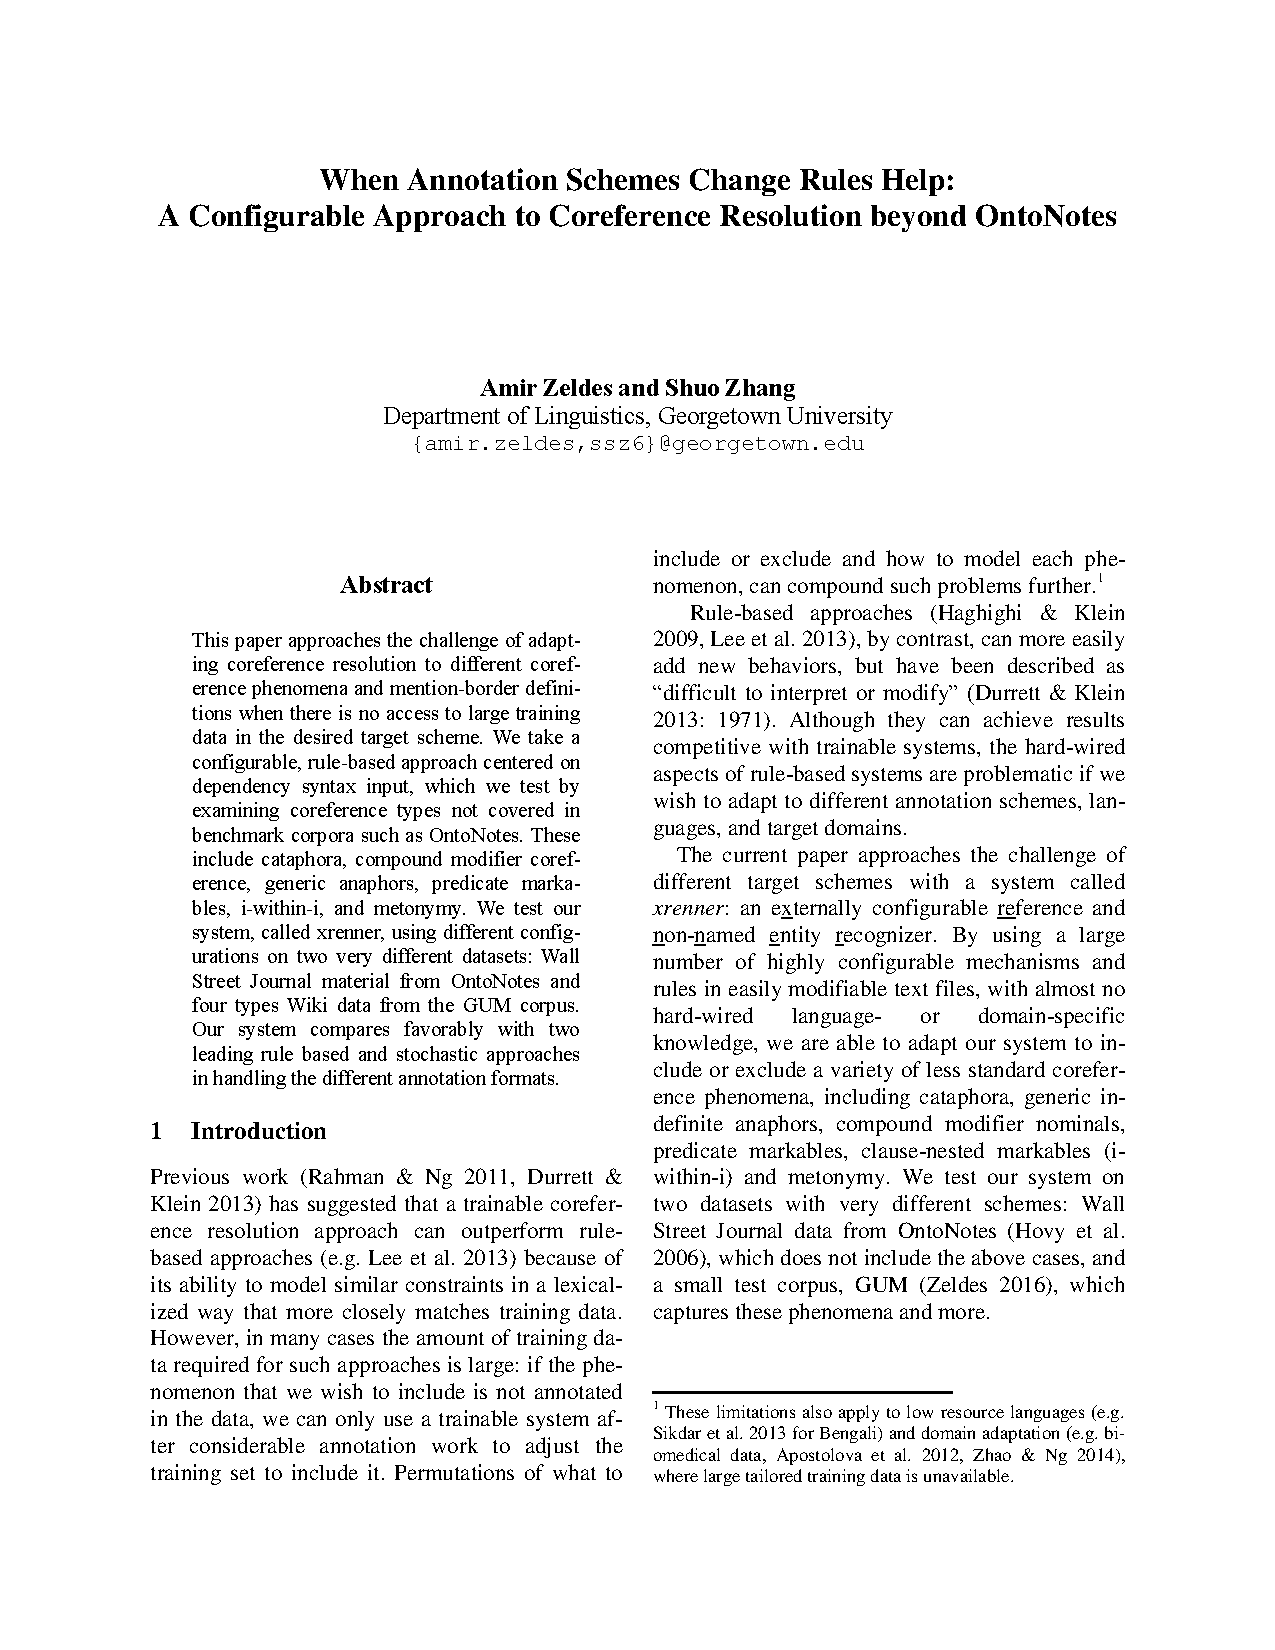
\includepdf[pages=1,addtotoc={1,chapter,1,{When Annotation Schemes Change Rules Help:  A Configurable Approach to Coreference Resolution beyond OntoNotes},ref:paper_9}]{final/9/9_Paper.pdf}
\ClearShipoutPicture
\includepdf[pages=2-]{final/9/9_Paper.pdf}
   % automatically generated from DB file

% -------- END MATTER: AUTHOR INDEX --------

\ifthenelse{\equal{\draftflag}{1}}{}{
  \ifthenelse{\isodd{\value{page}}}{}
    {\newpage \thispagestyle{empty} \phantom{.}}
  \pagestyle{empty}
  \printindex
}

\end{document}
